\documentclass[12pt]{article}

% Packages
\usepackage[margin=1in]{geometry}
\usepackage{amsmath, amsthm, amssymb, physics, graphicx, pdfpages}

% Problem Box
\setlength{\fboxsep}{4pt}
\newsavebox{\savefullbox}
\newenvironment{fullbox}{\begin{lrbox}{\savefullbox}\begin{minipage}{\dimexpr\textwidth-2\fboxsep\relax}}{\end{minipage}\end{lrbox}\begin{center}\framebox[\textwidth]{\usebox{\savefullbox}}\end{center}}
\newenvironment{pbox}[1][]{\begin{fullbox}\ifx#1\empty\else\paragraph{#1}\fi}{\end{fullbox}}

% Options
\allowdisplaybreaks
\addtolength{\jot}{1em}
\theoremstyle{definition}
\setlength{\parindent}{0pt}
\setlength{\parskip}{6pt}

% Default Commands
\newtheorem{proposition}{Proposition}
\newtheorem{lemma}{Lemma}
\newcommand{\ds}{\displaystyle}
\newcommand{\isp}[1]{\quad\text{#1}\quad}
\newcommand{\N}{\mathbb{N}}
\newcommand{\Z}{\mathbb{Z}}
\newcommand{\Q}{\mathbb{Q}}
\newcommand{\R}{\mathbb{R}}
\newcommand{\C}{\mathbb{C}}
\newcommand{\eps}{\varepsilon}
\renewcommand{\phi}{\varphi}
\renewcommand{\emptyset}{\varnothing}

% Extra Commands


% Document Info
\title{\vspace{-0.5in}Lab 4 \\
    \large GEOG 191
}
\author{Harry Coleman}
\date{February 12, 2021}

% Begin Document
\begin{document}
\maketitle


\section{Cost}
\subsection{Code}
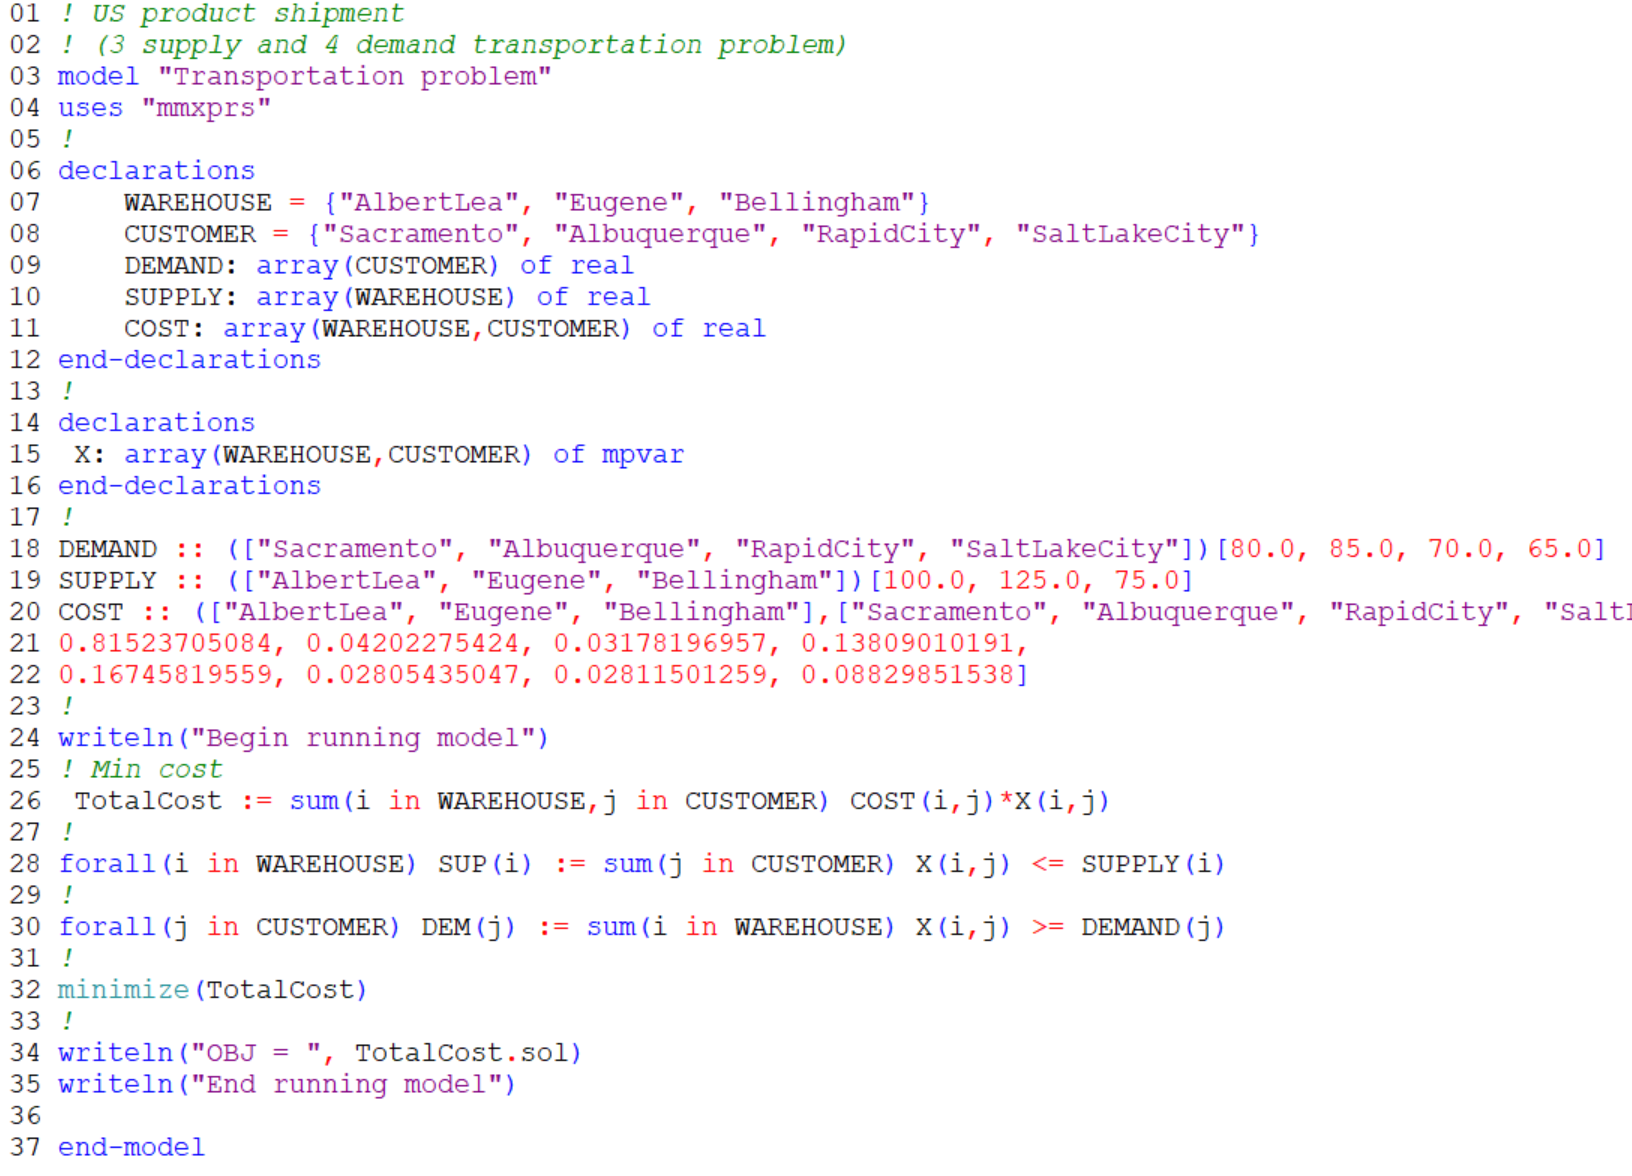
\includegraphics[width=\textwidth]{codecost.png}
\newpage
\subsection{Cost  Values}
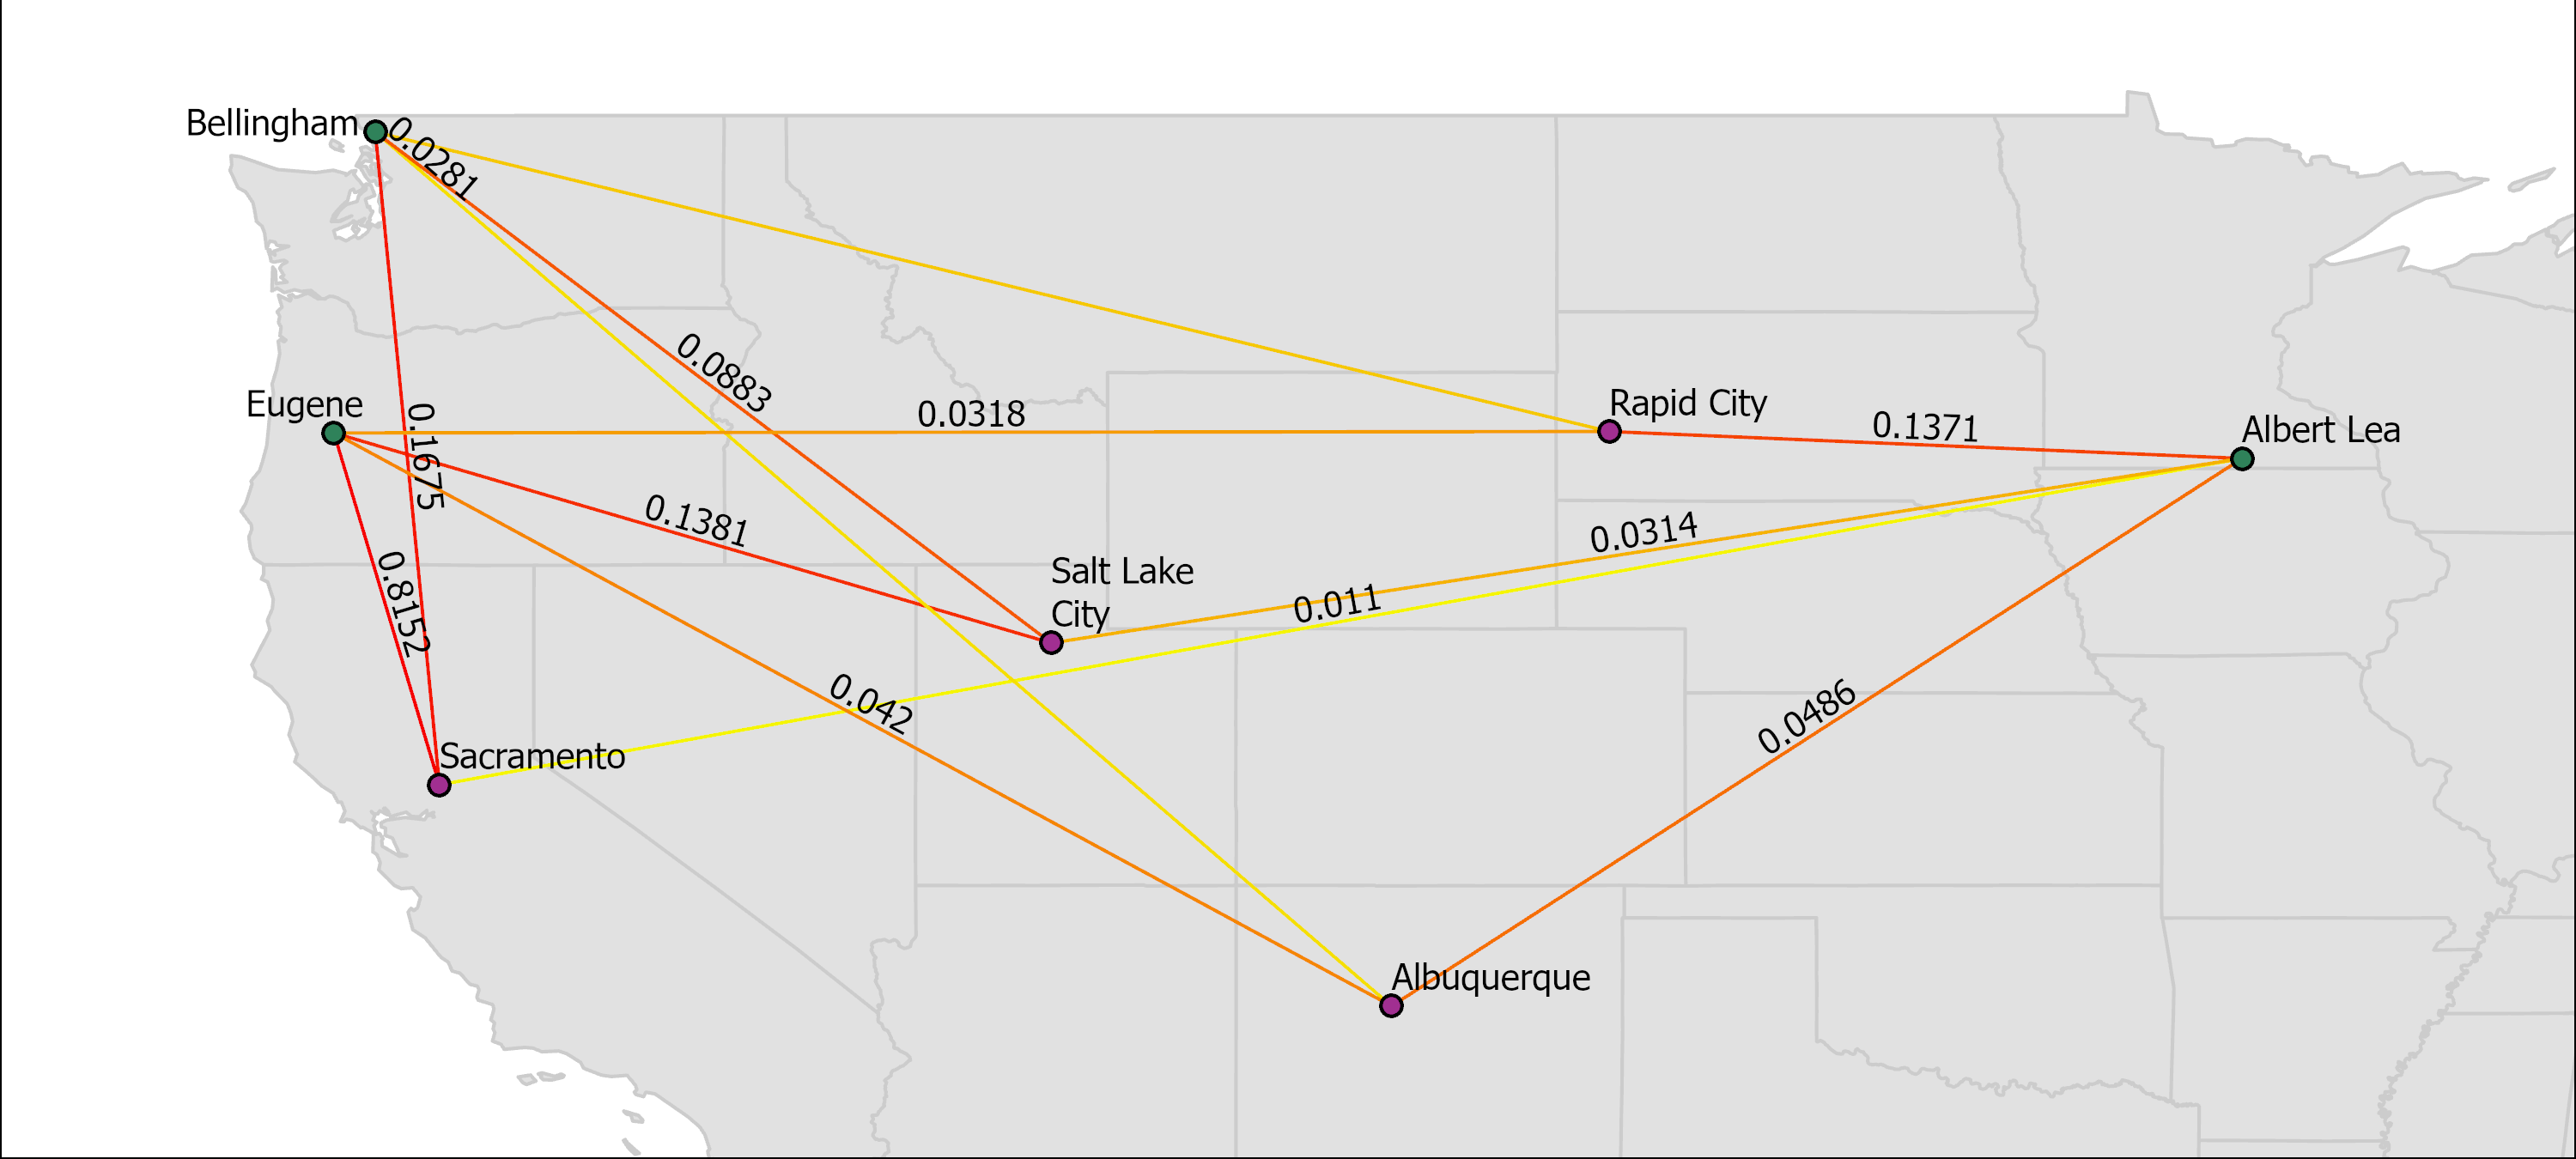
\includegraphics[width=\textwidth]{mapcost.png}
\subsection{Allotments}
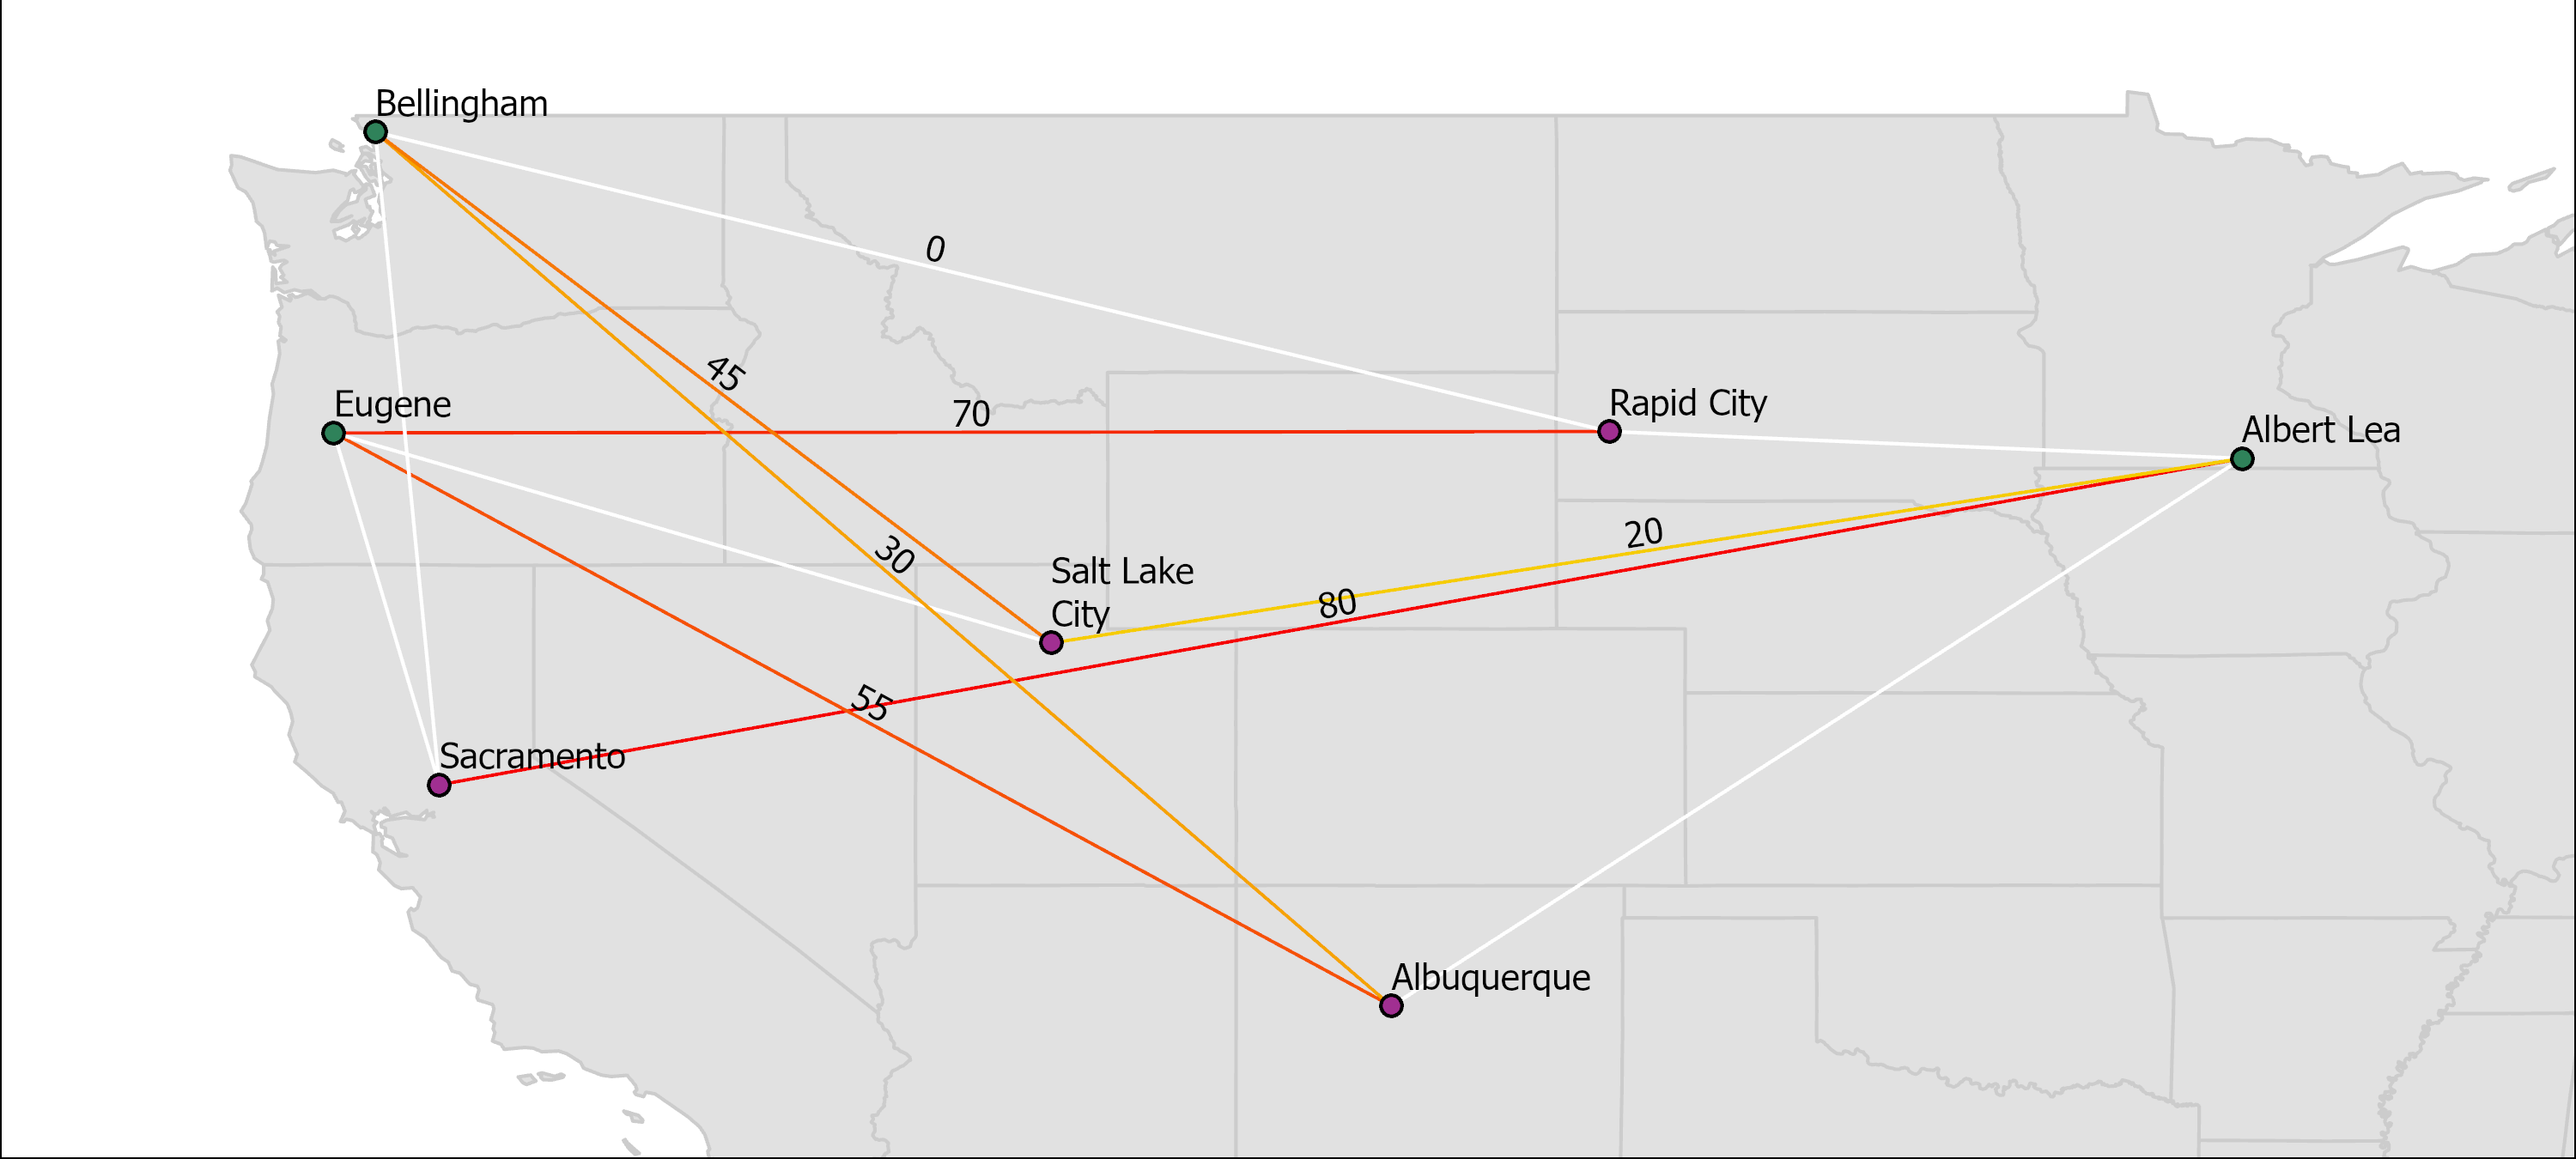
\includegraphics[width=\textwidth]{solmapcost.png}

Total Cost: $10.85982568$

\newpage
\section{Interact}
\subsection{Code}
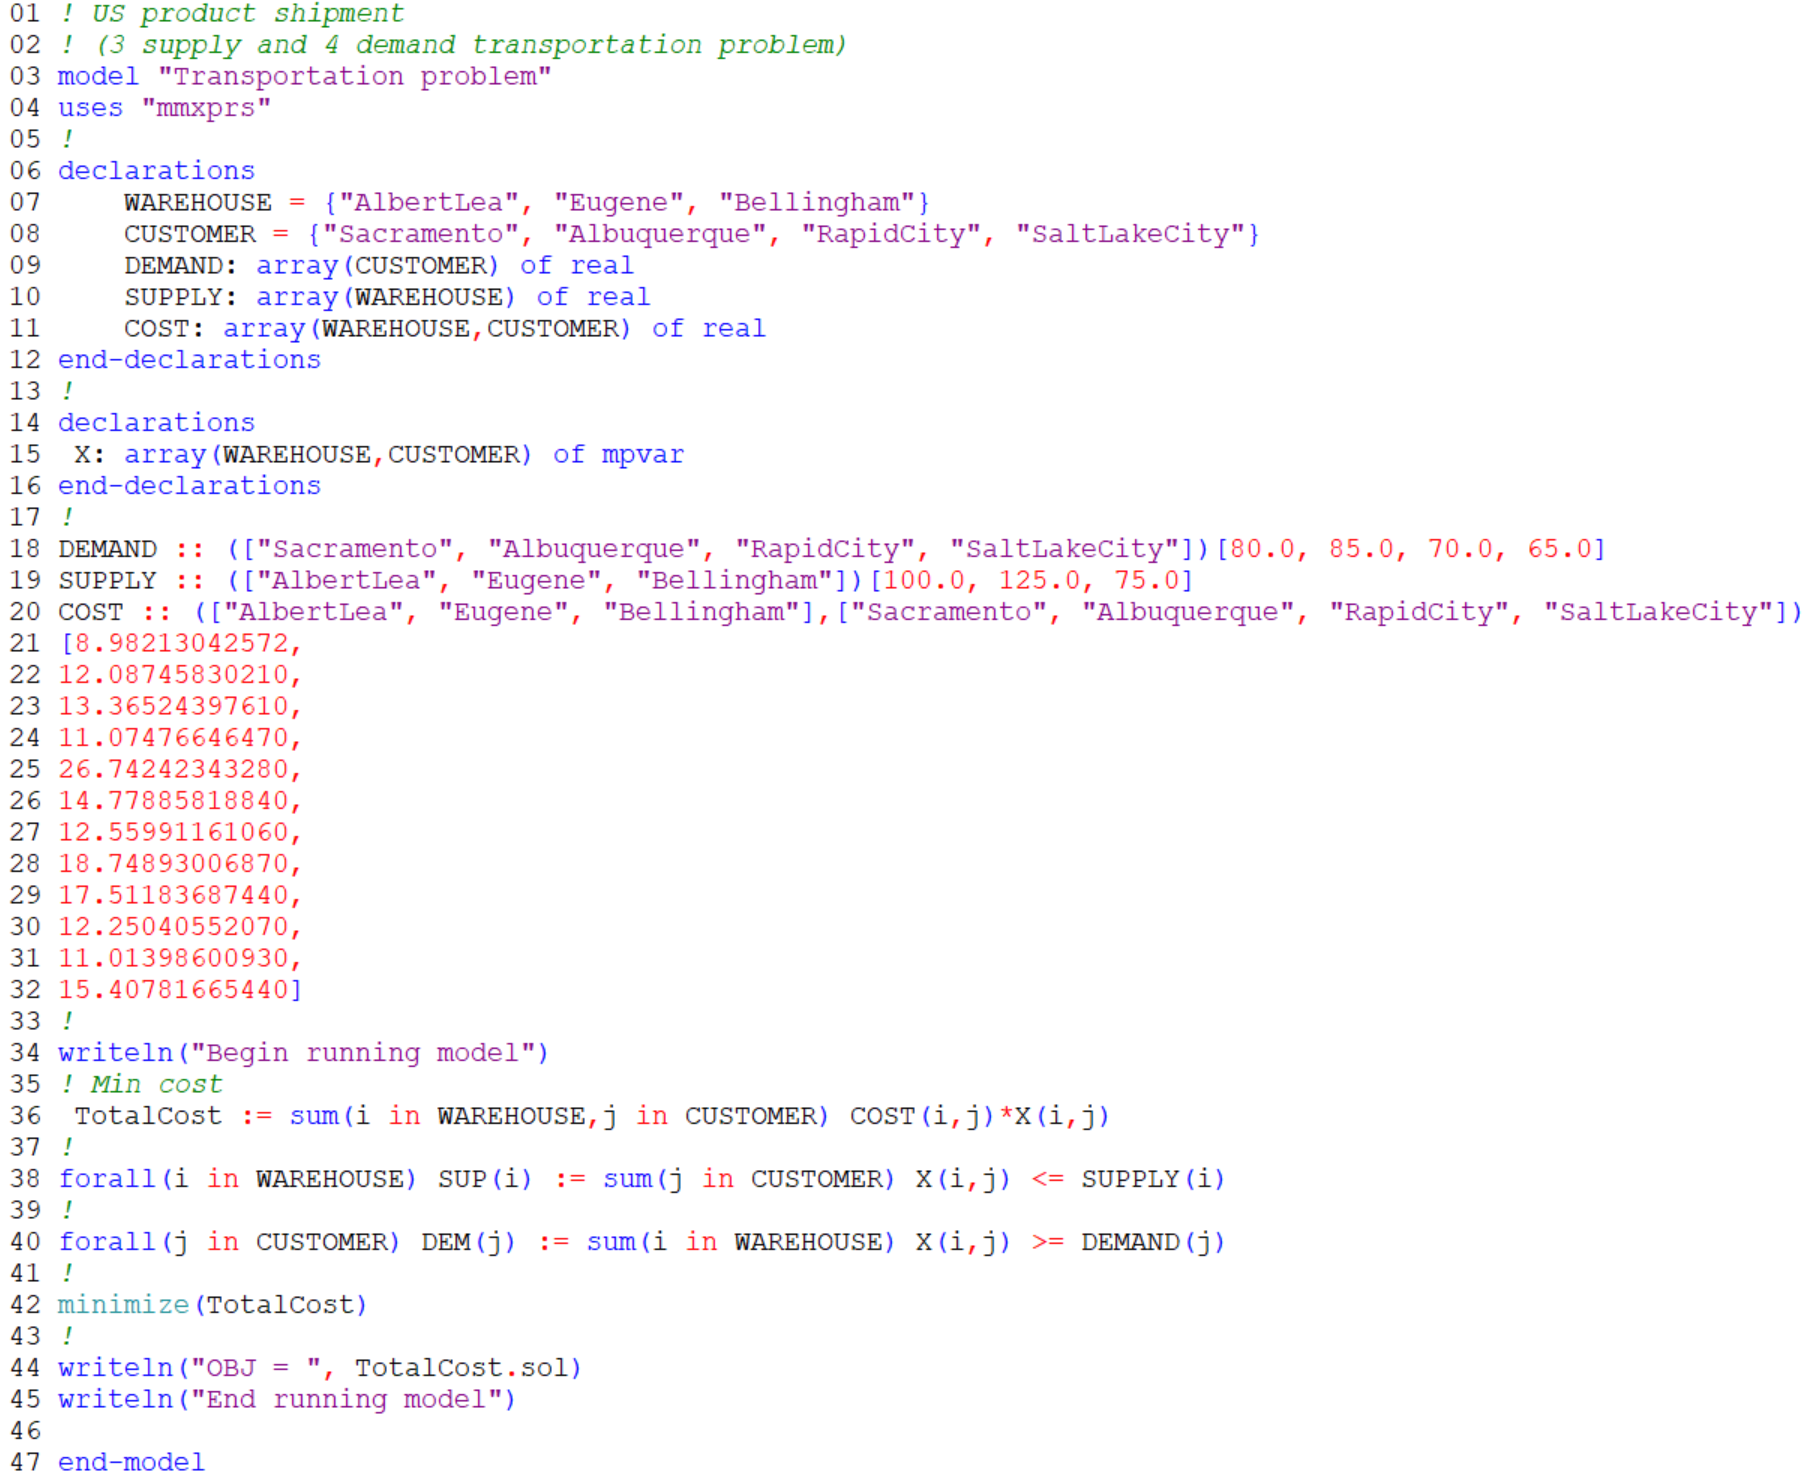
\includegraphics[width=\textwidth]{codeint.png}
\newpage
\subsection{Interact Values}
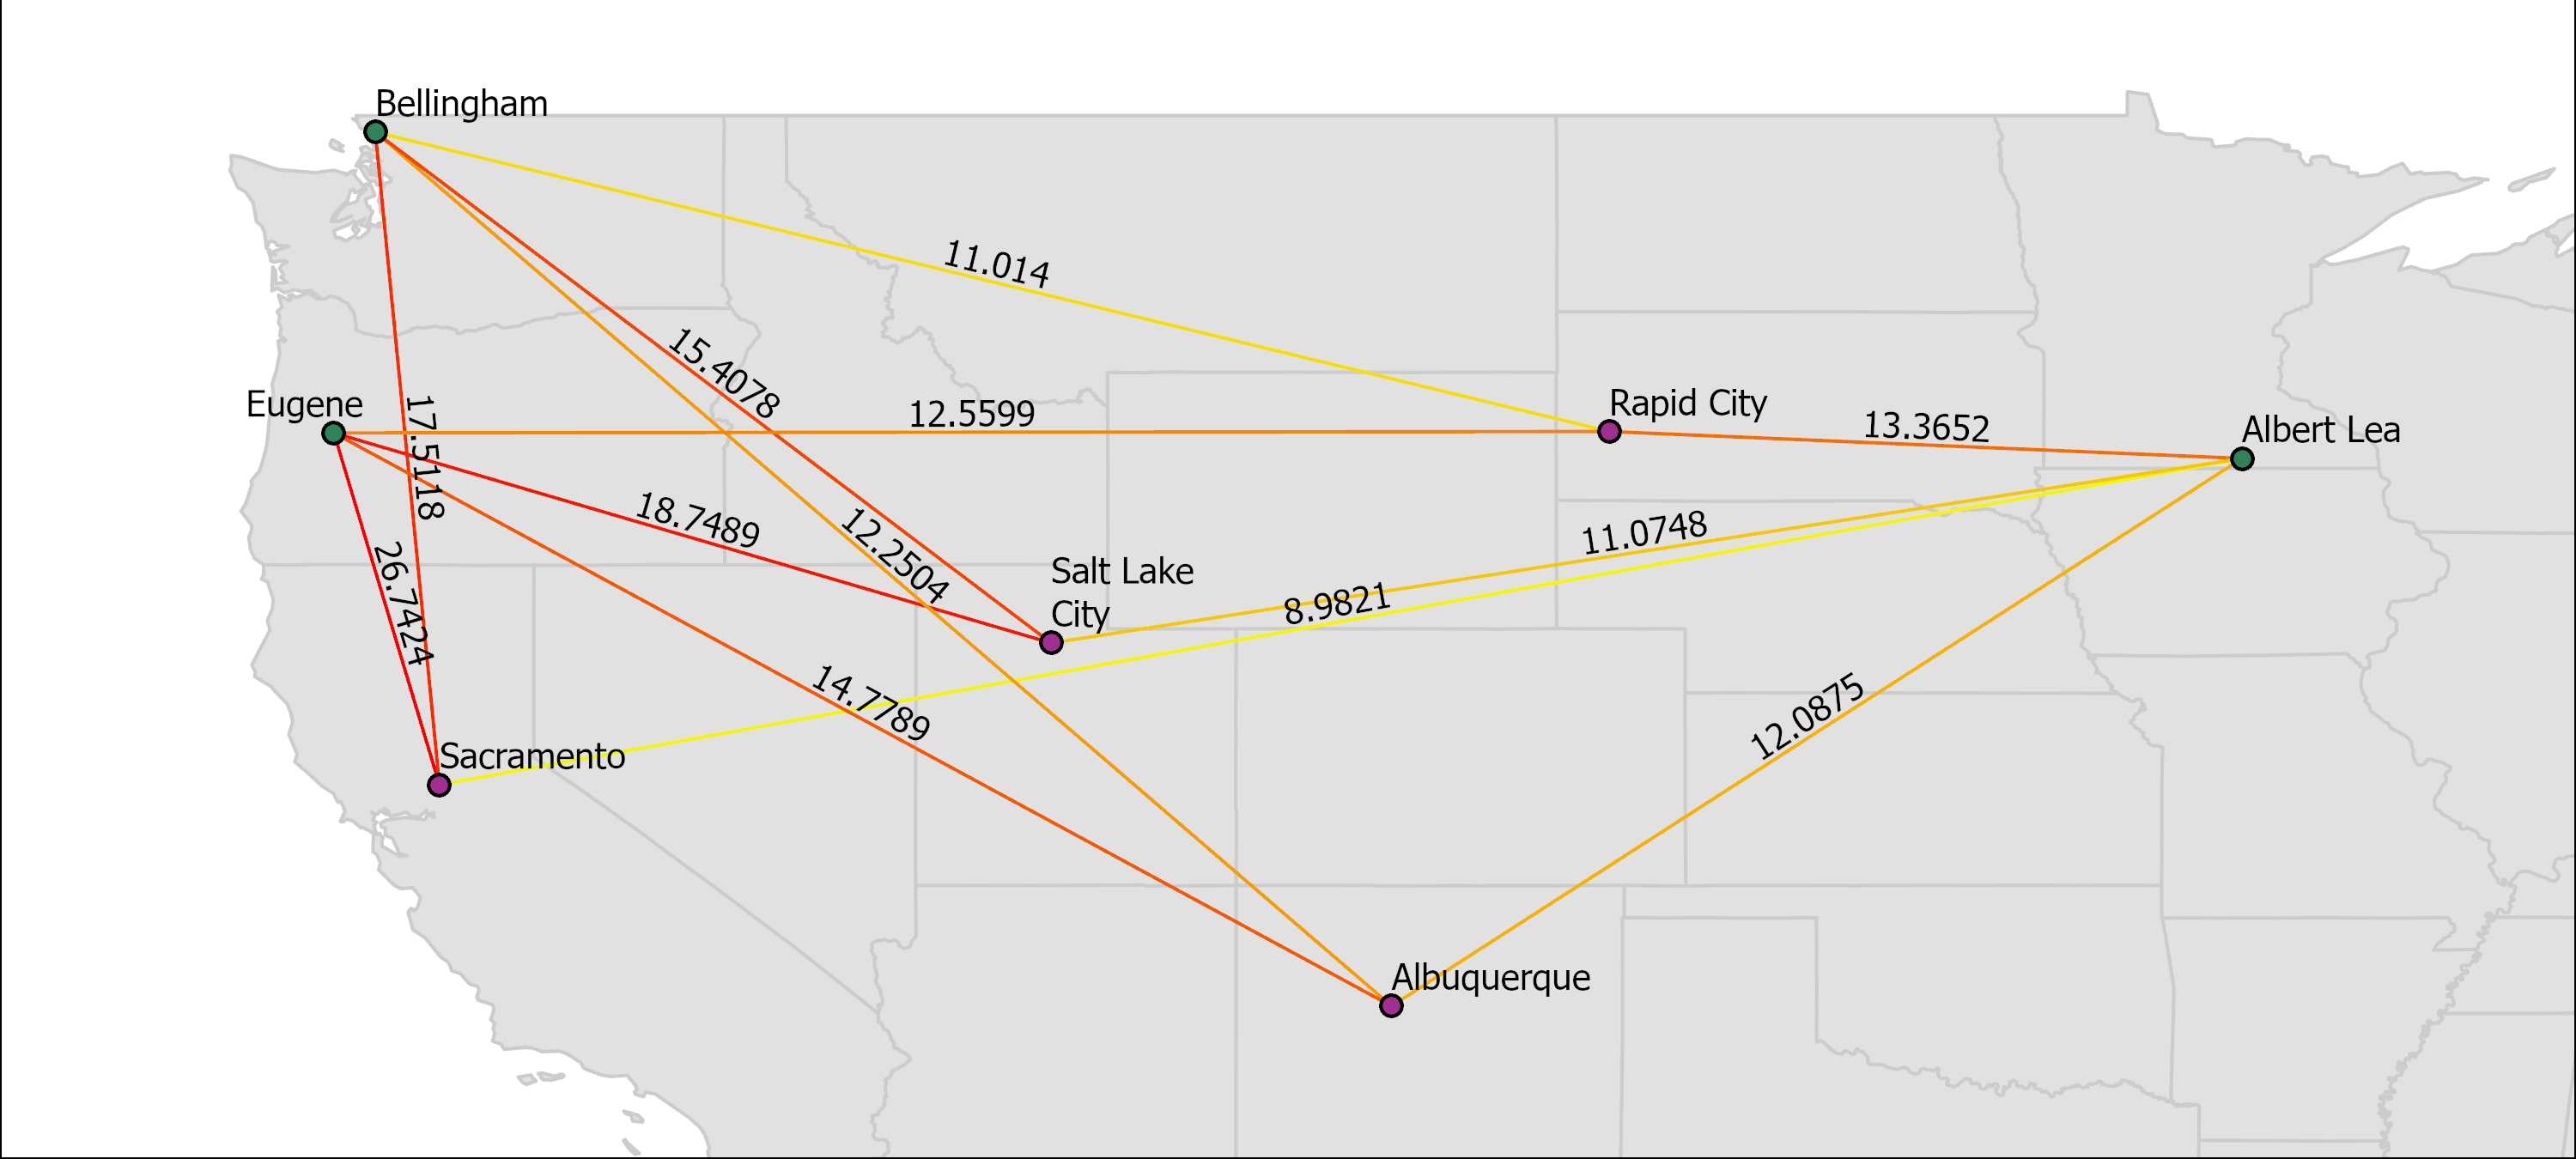
\includegraphics[width=\textwidth]{mapint.png}
\subsection{Allotments}
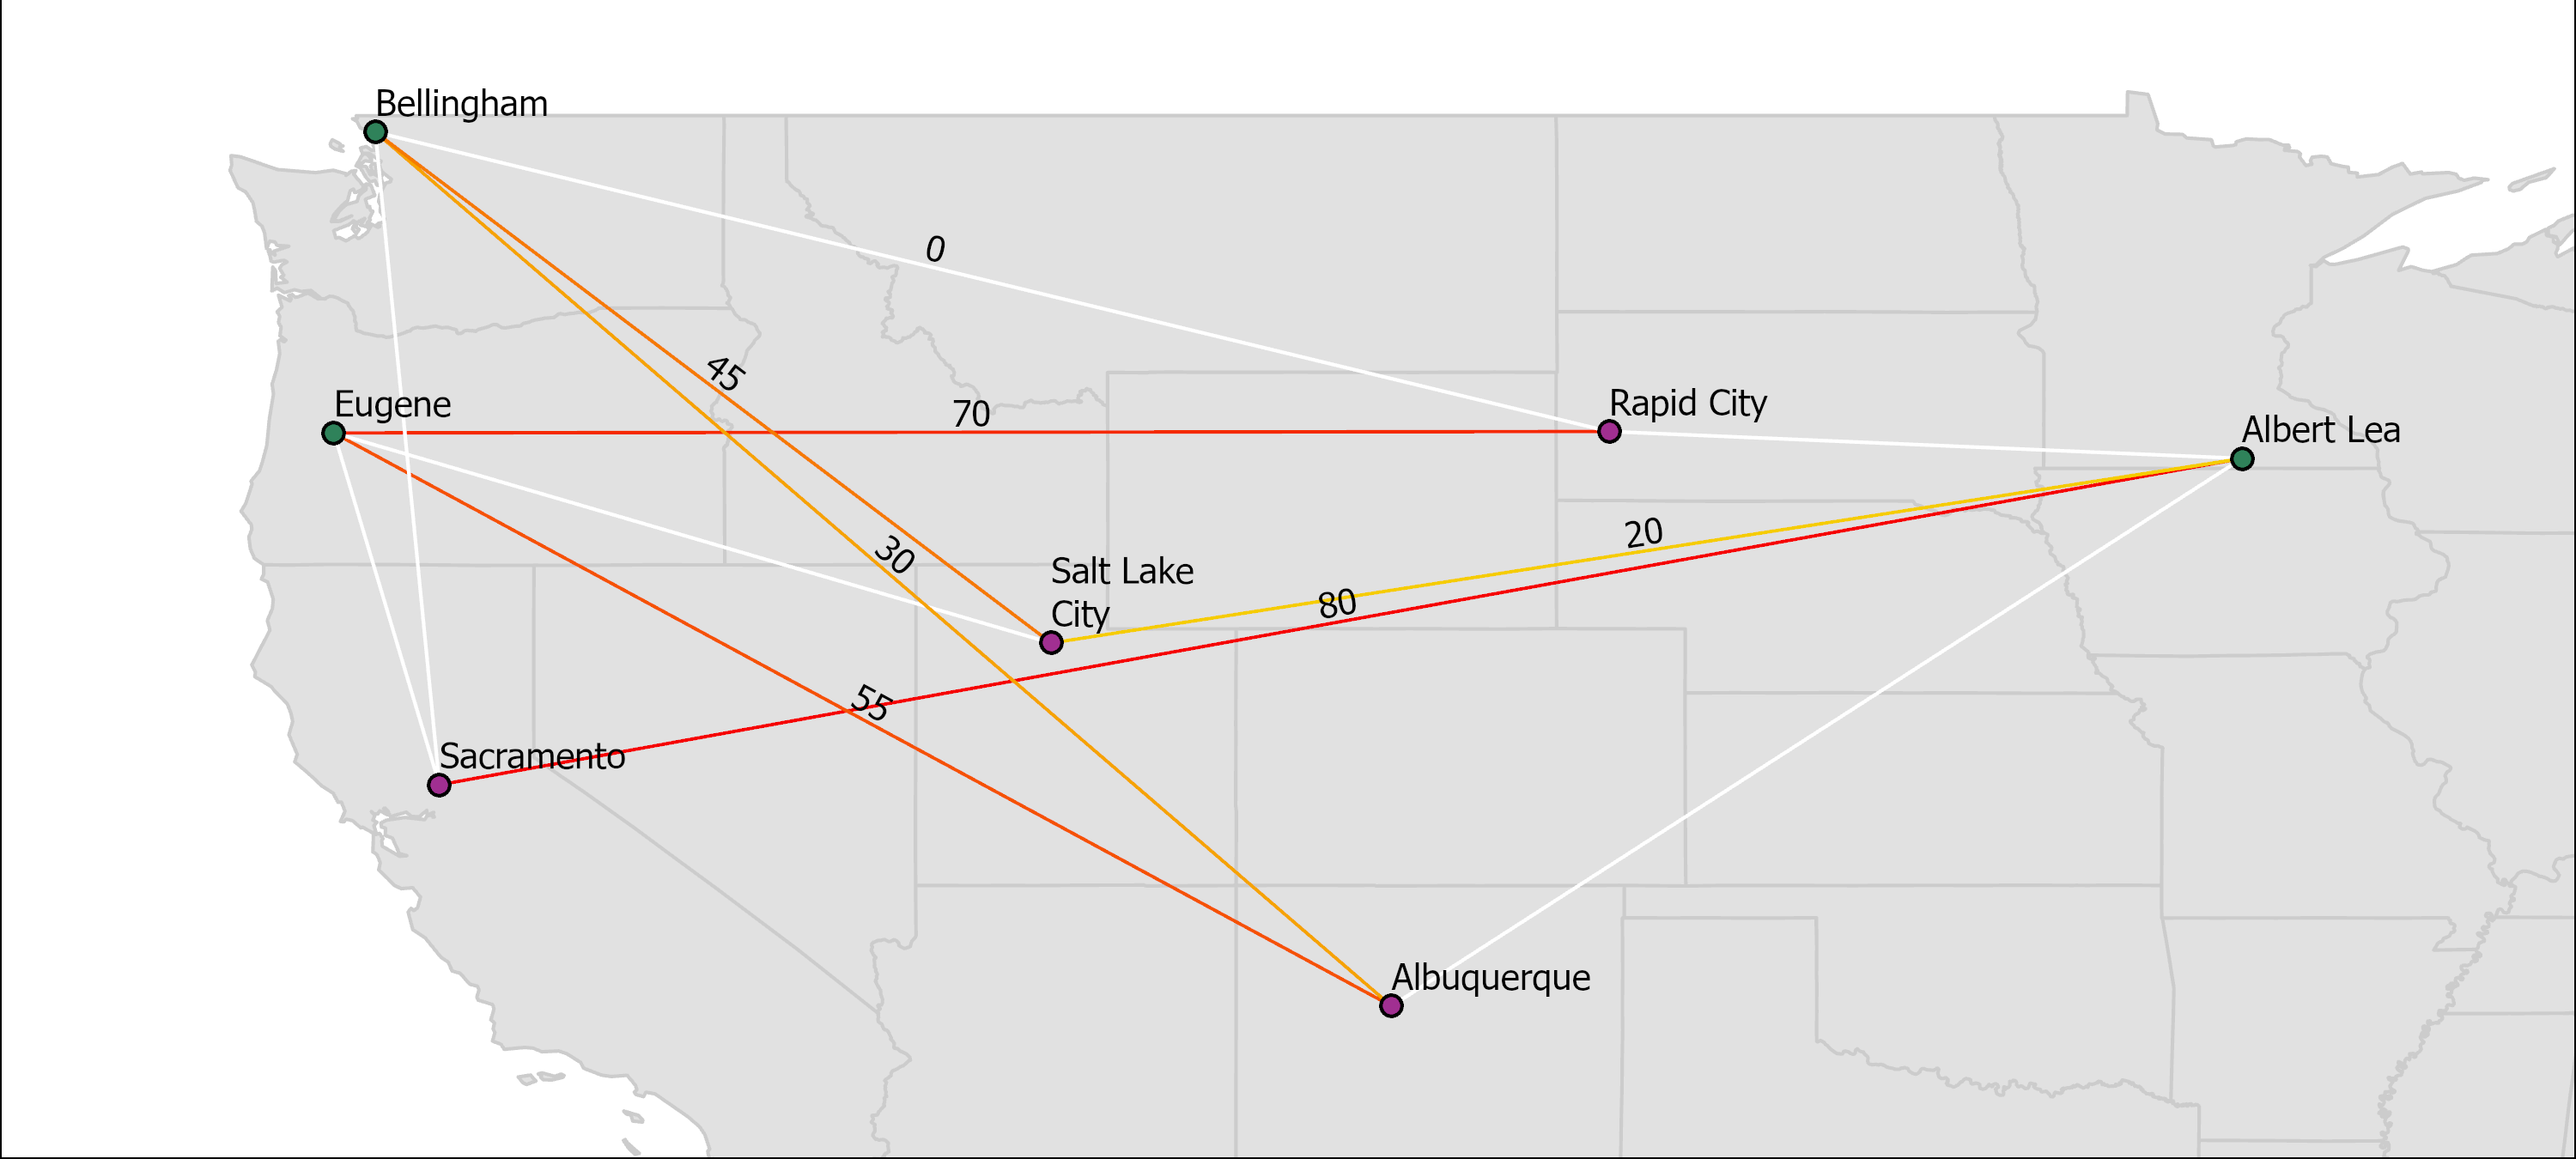
\includegraphics[width=\textwidth]{solmapcost.png}

Total Interact: $3692.960692$

\newpage
\section{Dist}
\subsection{Code}
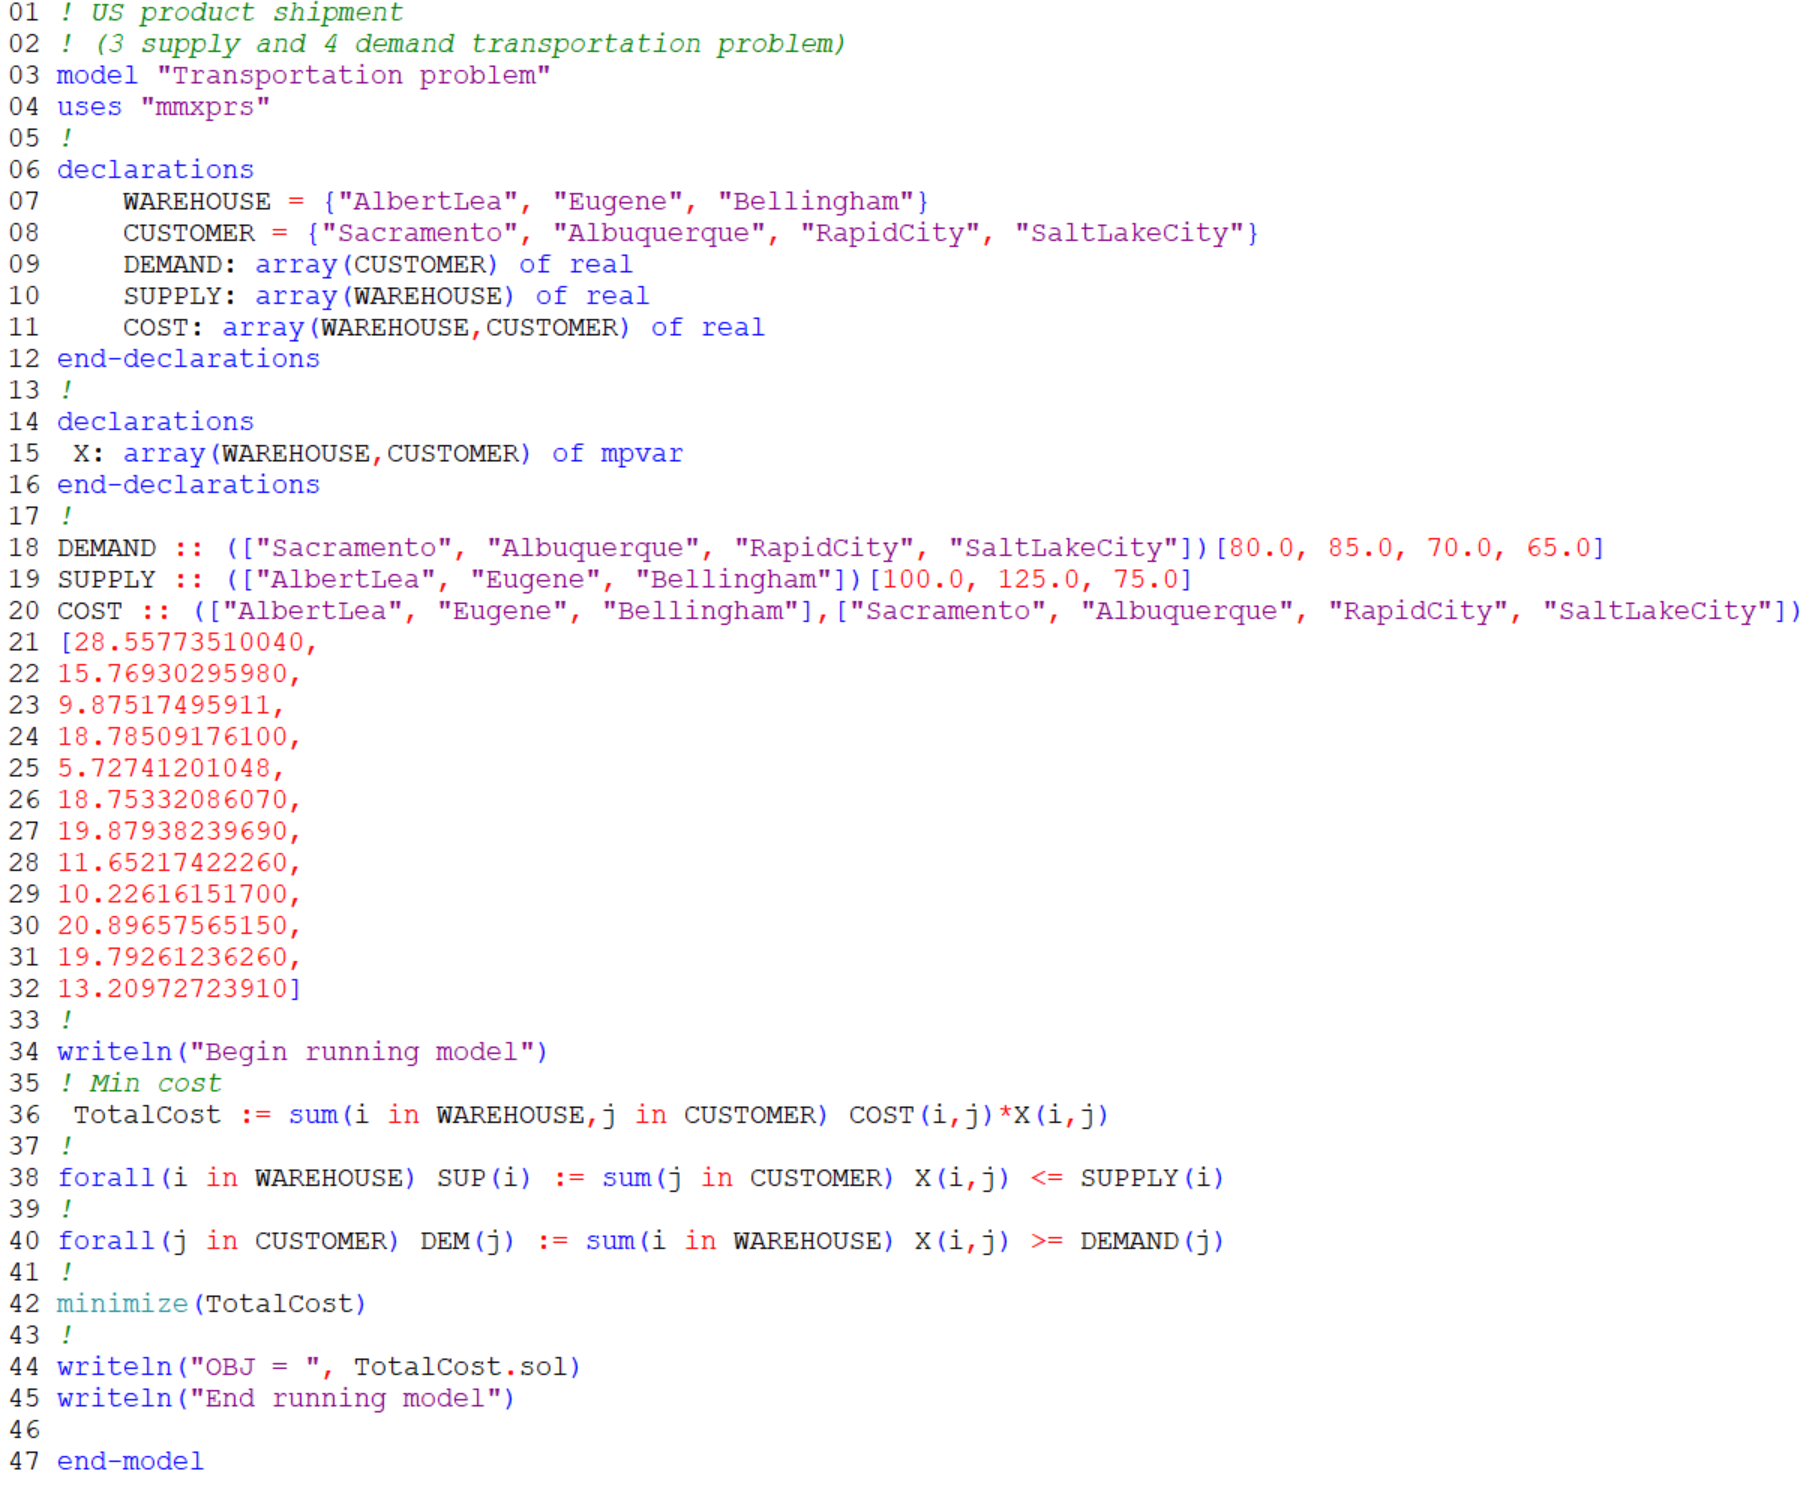
\includegraphics[width=\textwidth]{codedist.png}
\newpage
\subsection{Dist Values}
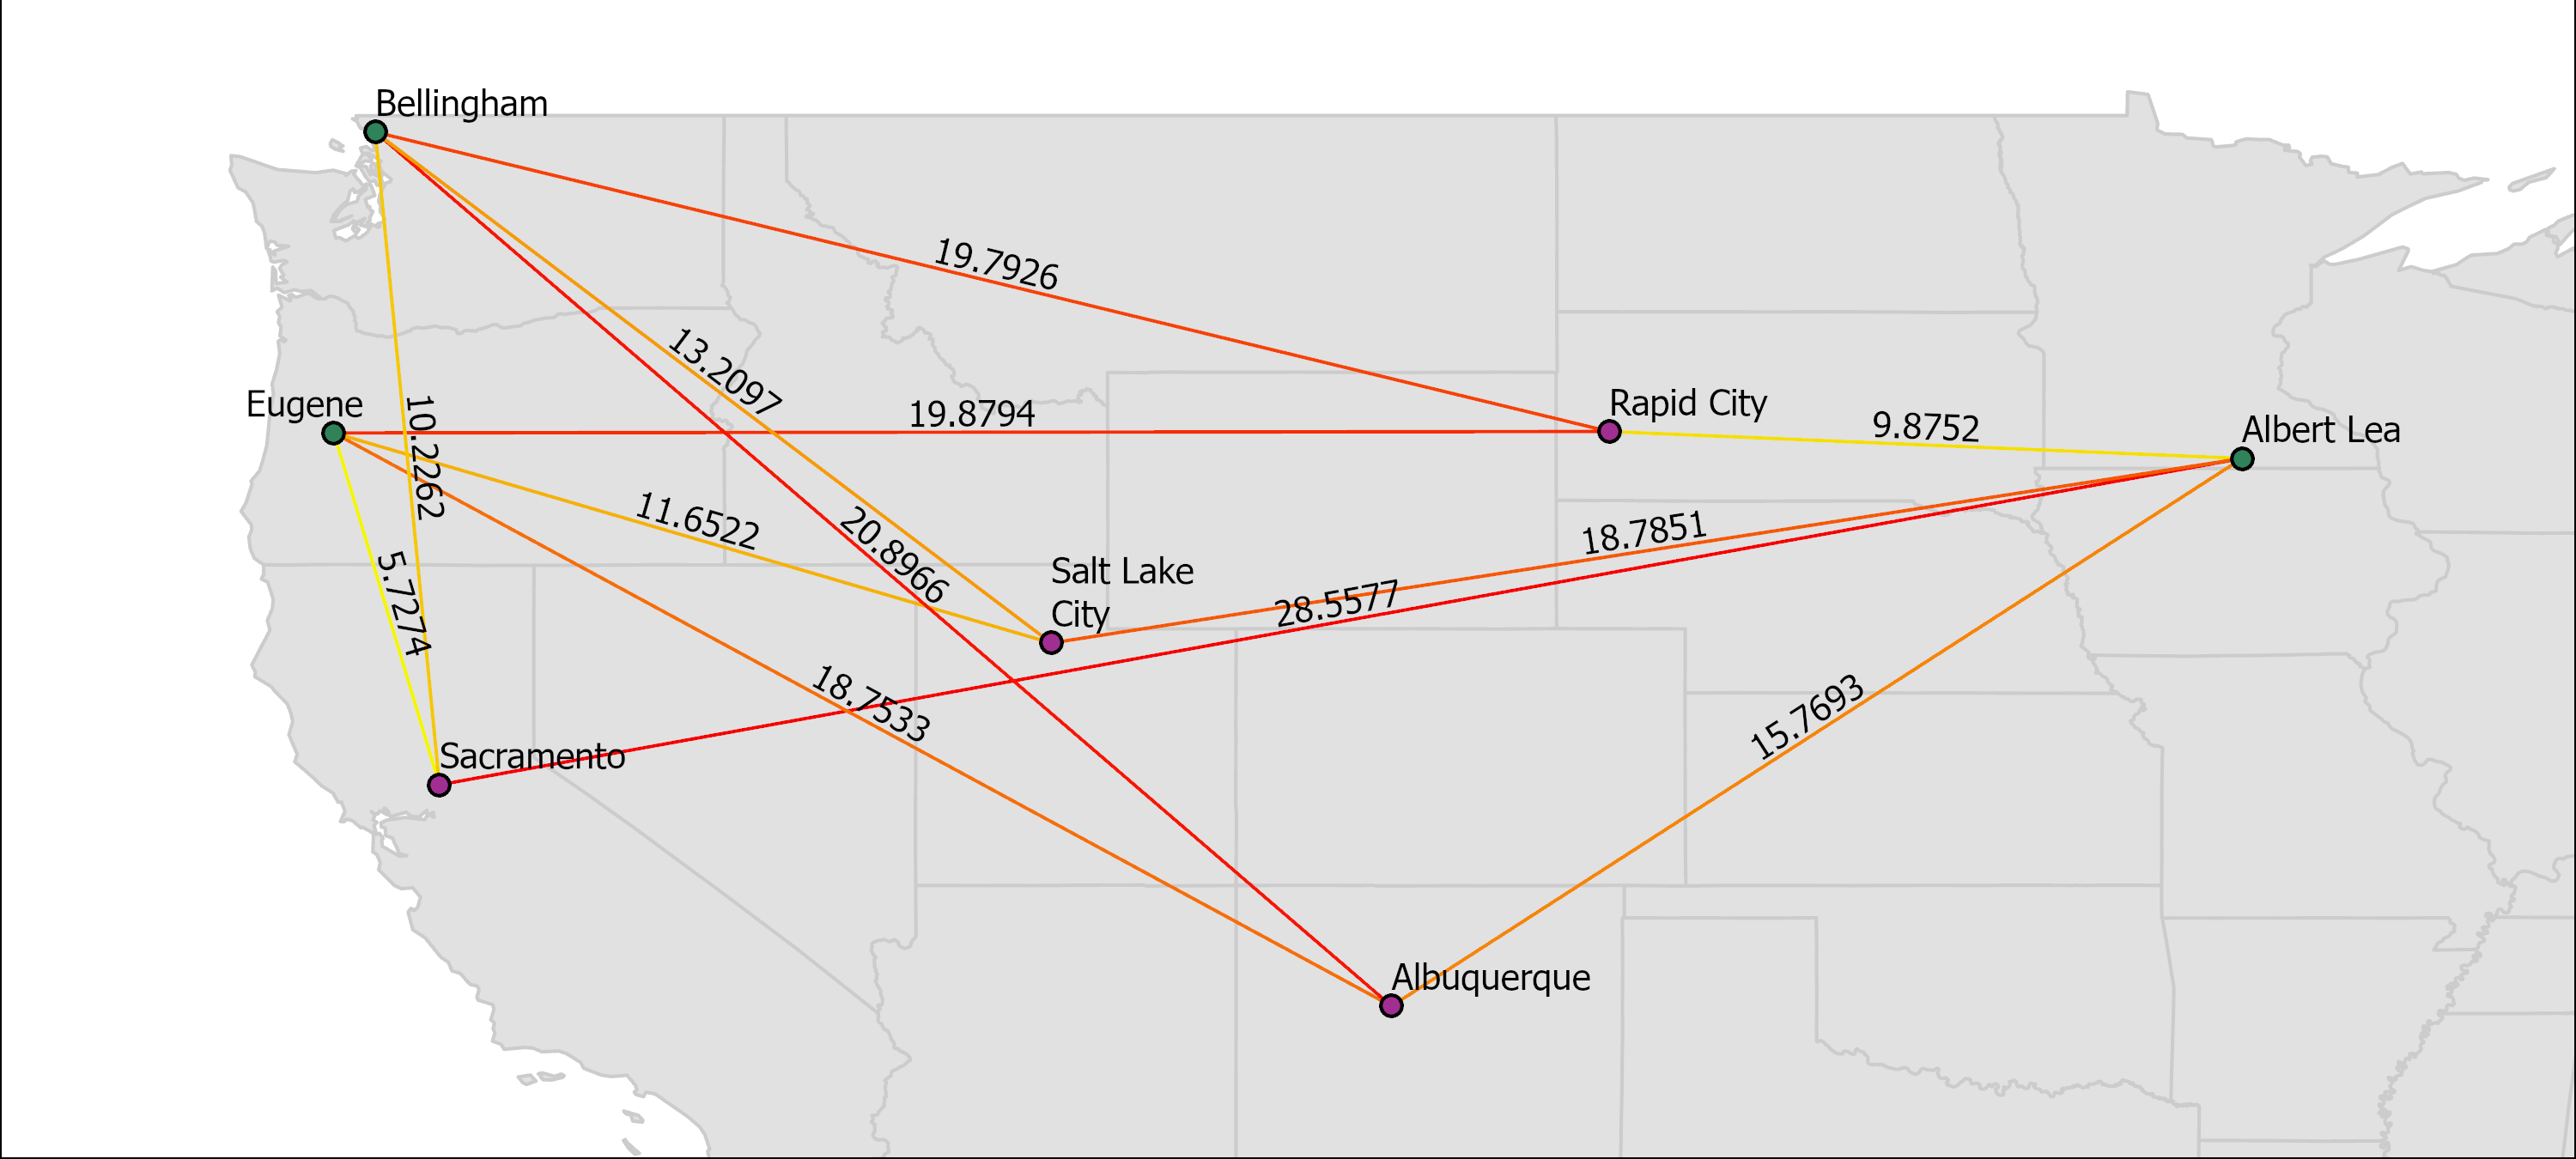
\includegraphics[width=\textwidth]{mapdist.png}
\subsection{Allotments}
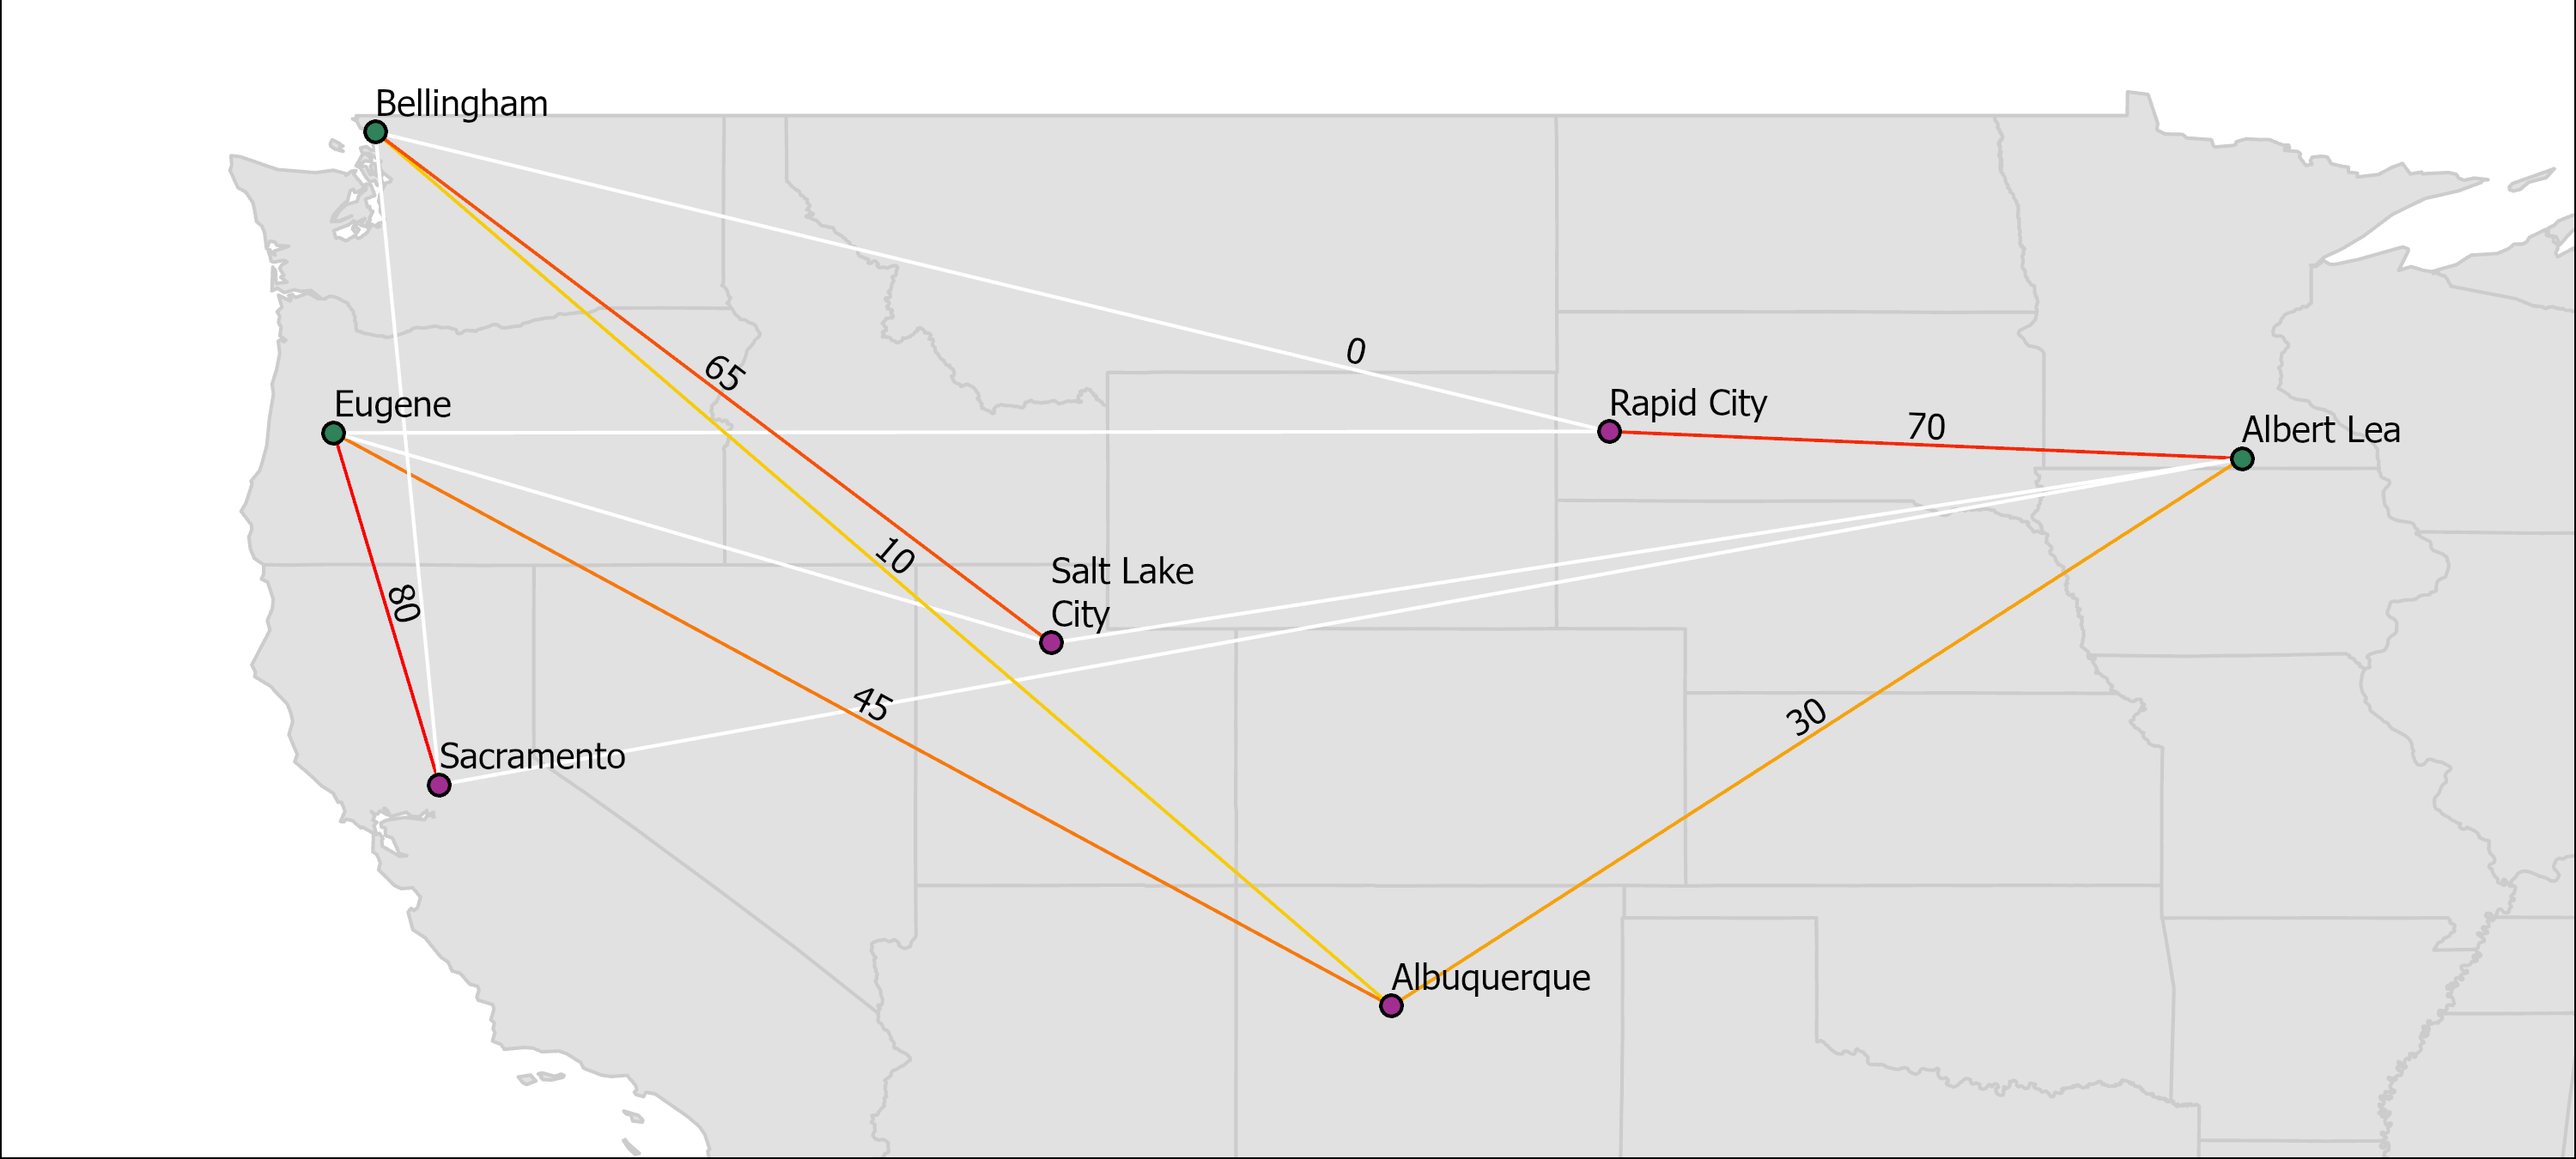
\includegraphics[width=\textwidth]{solmapdist.png}

Total Dist: $3534.031763$

\newpage
\section{Length}
\subsection{Code}
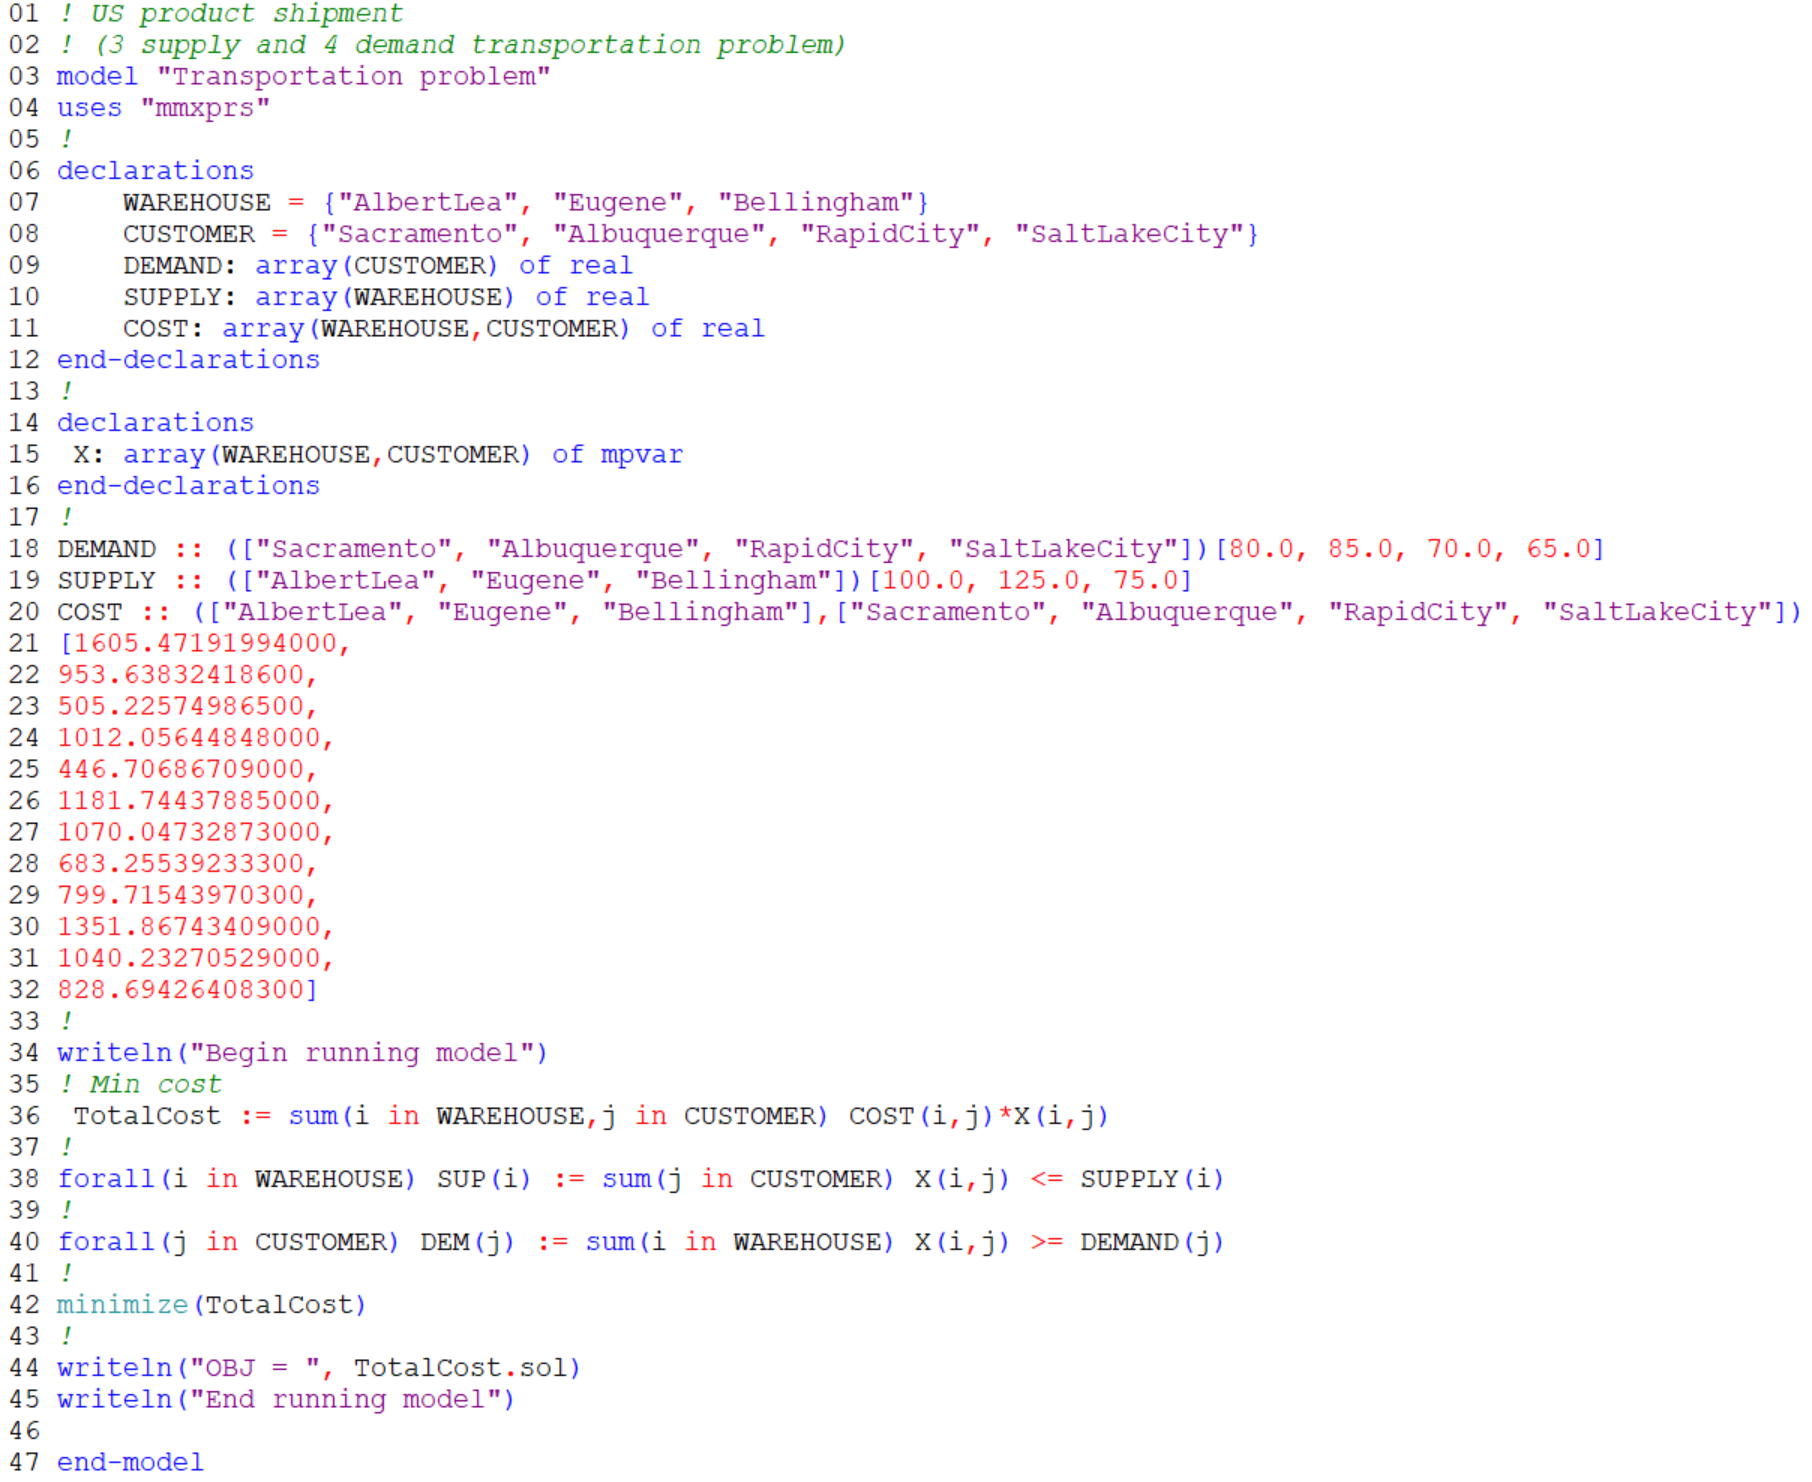
\includegraphics[width=\textwidth]{codelen.png}
\newpage
\subsection{Length Values}
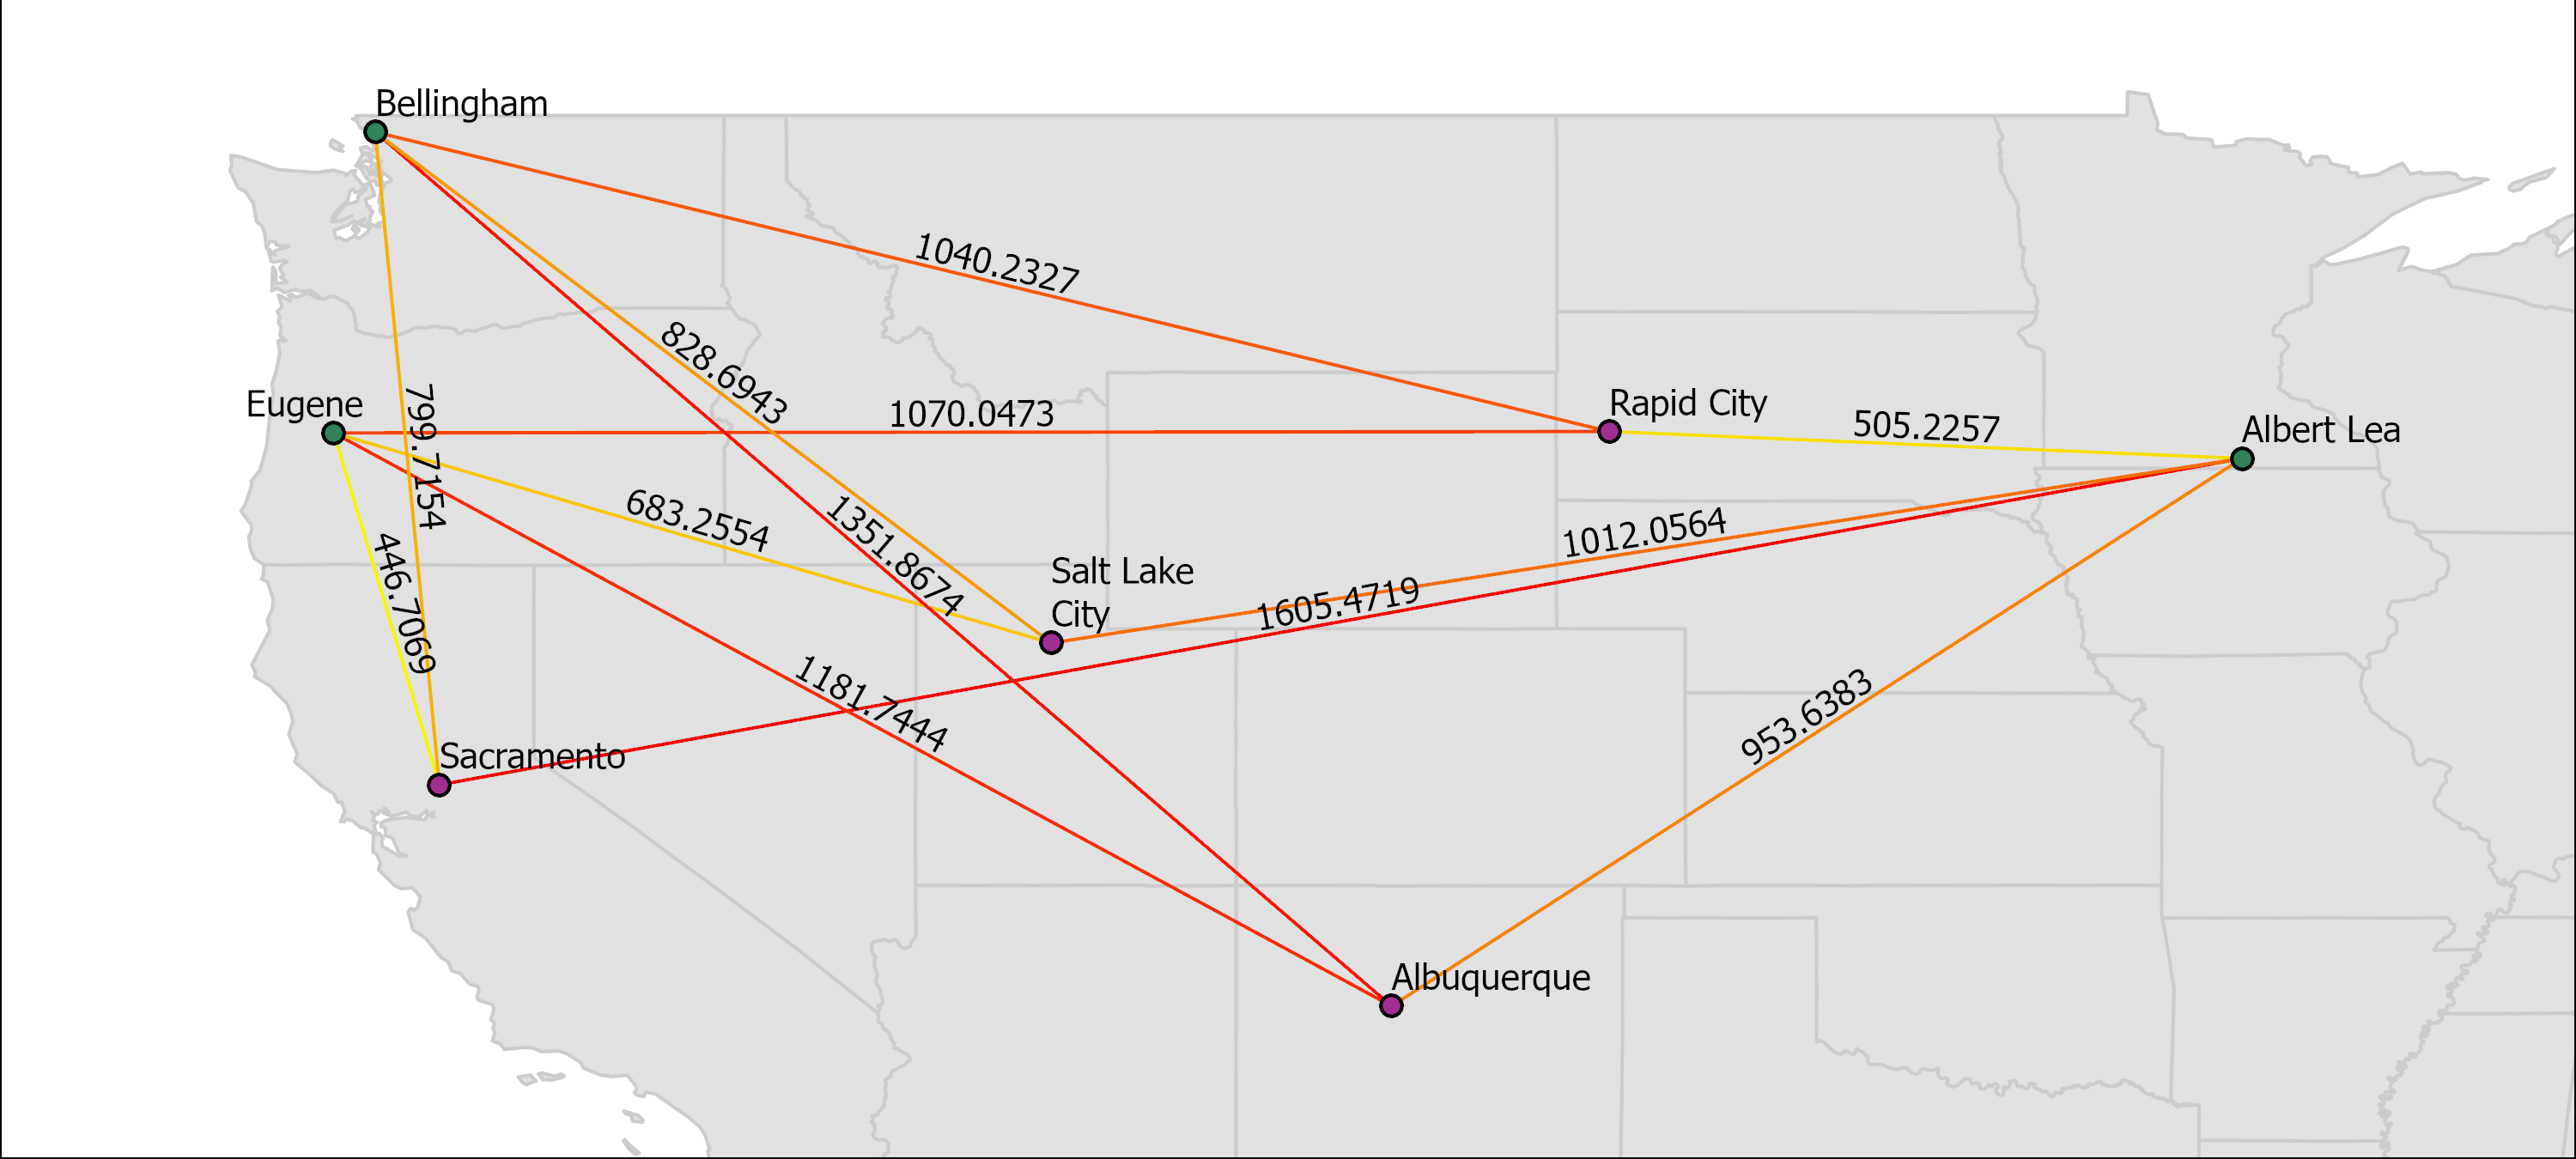
\includegraphics[width=\textwidth]{maplen.png}
\subsection{Allotments}
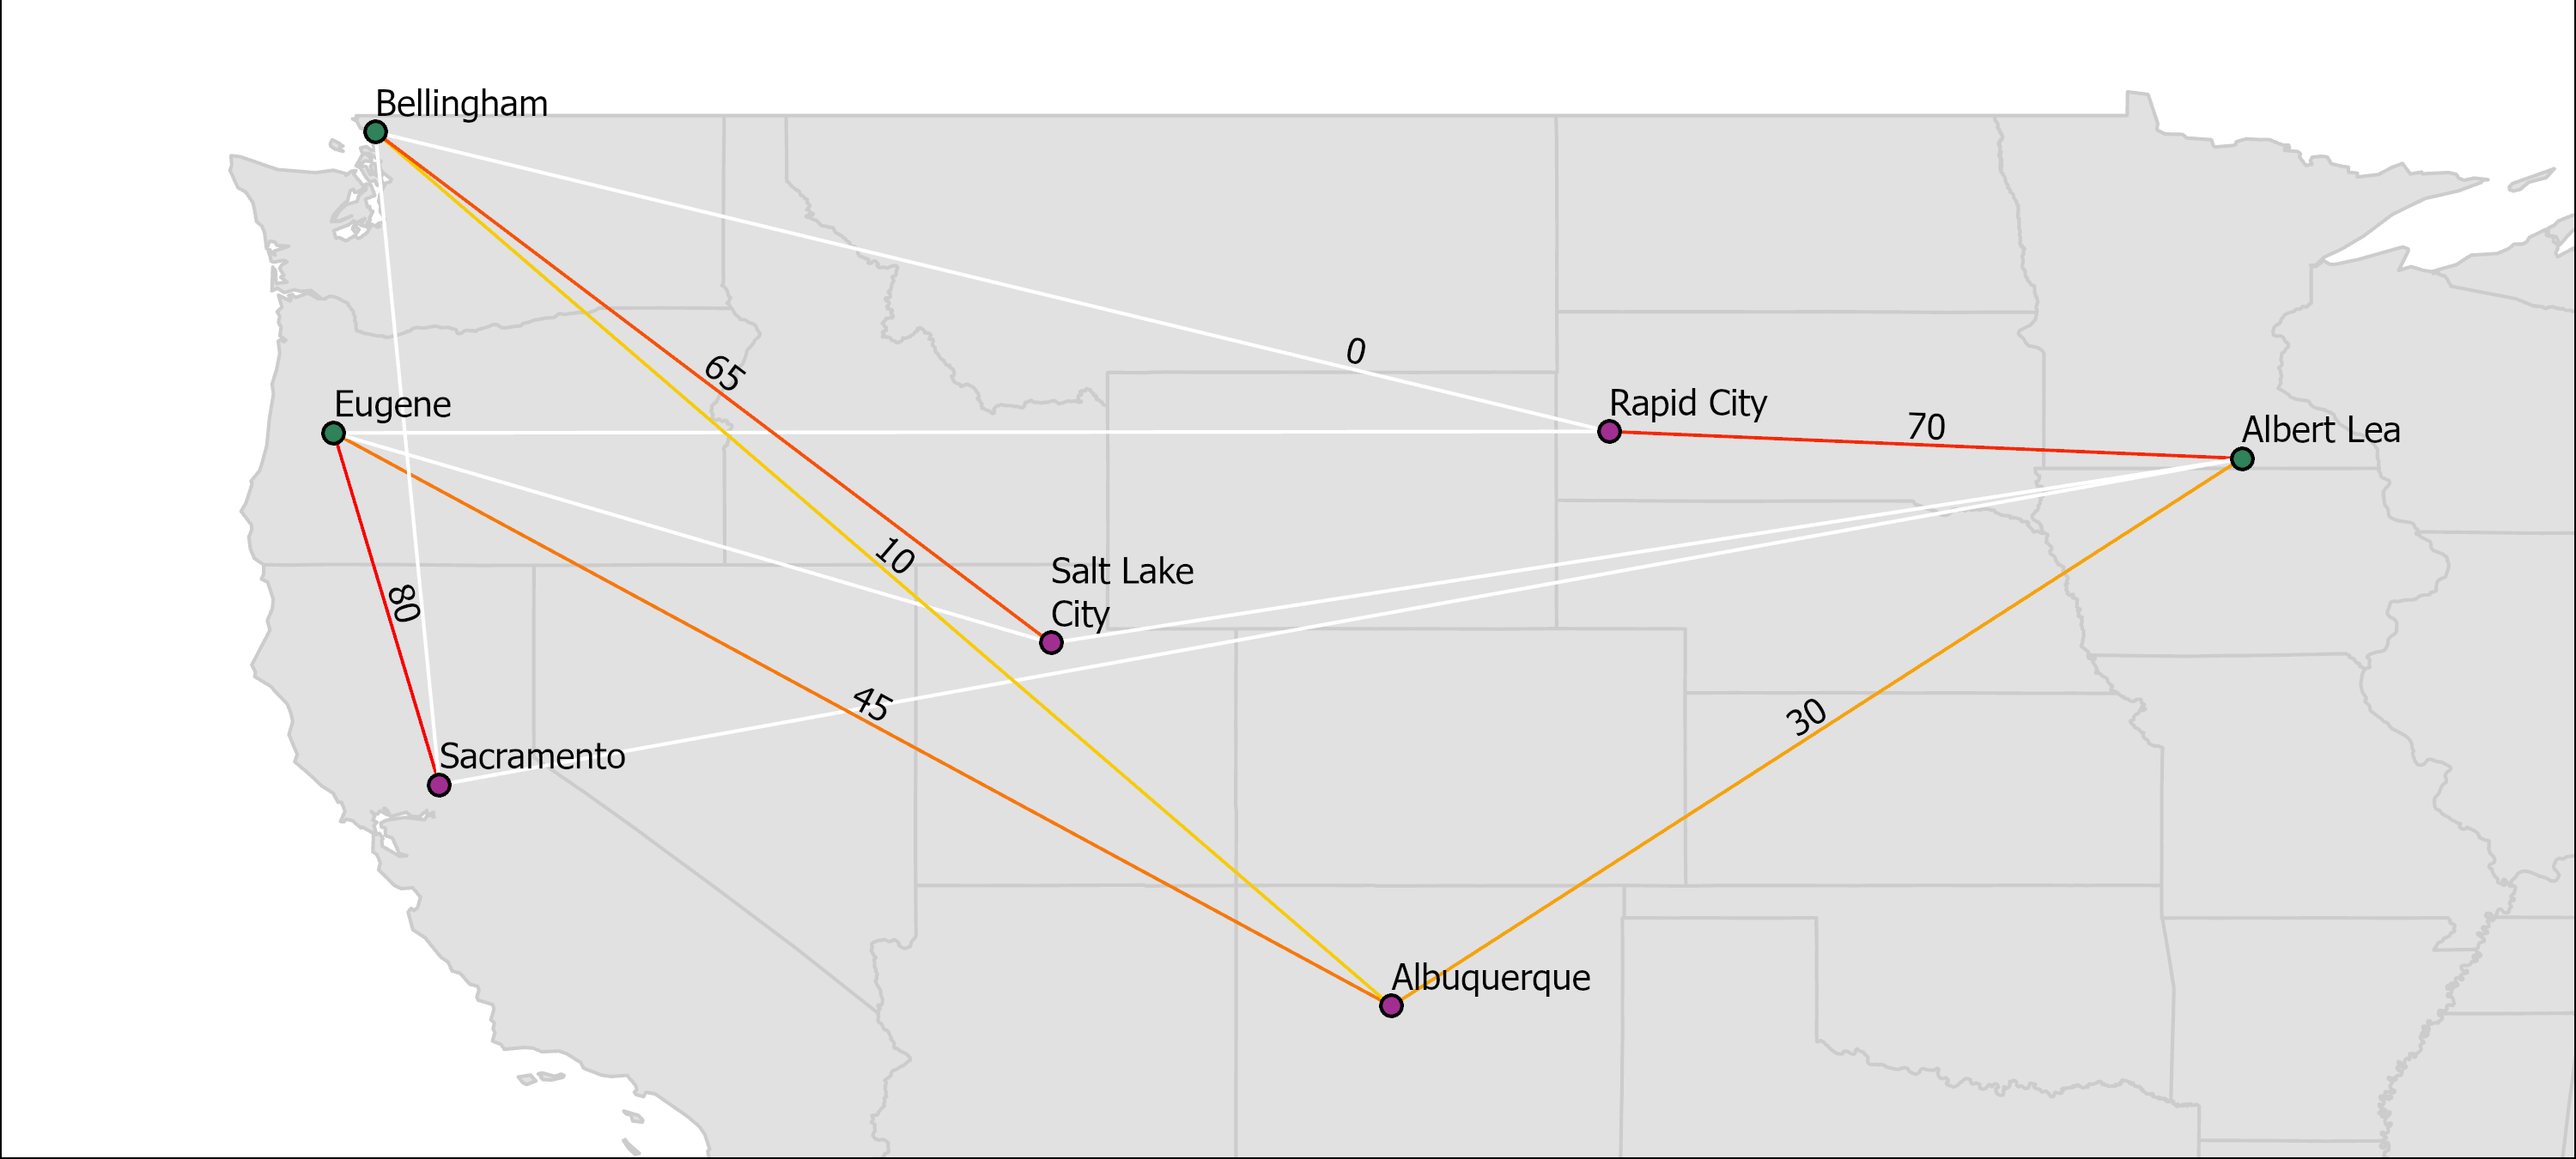
\includegraphics[width=\textwidth]{solmapdist.png}

Total Length: $220273.8001$

\newpage
\section{Observations}

In all instances, Xpress produced an optimal solution after 7 or 8 iterations of the simplex dual algorithm.

Both Cost and Interact produced identical solutions and, similarly, Dist and Length produced identical solutions.

Since our goal is is to minimize the objective value, a route is more likely to be allotted units when its corresponding objective coefficient is smaller. Consider the route from Albert Lea to Rapid City. This route has Cost and Interact values in the upper ranges over all routes, as indicated by both the number and color. As we might expect, this route was allotted no units in both cases. On the other hand, this route has Dist and Length values in the lower ranges over all routes, and ends up being allotted a large number of units.

Another example of this would be the route from Eugene to Sacramento. With high Cost and Interact values, no units are allotted in either case. But with lower Dist and Length values, the route is allotted many units.

However, if we look at Albuquerque, it seems to break this rule. The supplier with the least Cost to Albuquerque is Bellingham, but this supplier ends up sending a minority of Albuquerque's demand, the rest of which comes from Eugene. And in terms of Interact, Albert Lea has the least value, but ends up sending no units to Albuquerque, at all. A similar situation results when considering both Dist and Length, with less than half of Albuquerque's units coming from the ``cheapest'' supplier.

This can be explained by following the route back to Albert Lea, which has a maximum supply of $100$ units. The route from Albert Lea to Sacramento has a very low Cost and Interact; the lowest of all routes, in fact. So, in both these cases, Albert Lea ends up sending all $80$ units that Sacramento demands, because of how cheap it is to do so. But this leaves Albert Lea with only $20$ additional units to send, which are directed towards Salt Lake City, rather than Albuquerque. And when we consider Dist and Length, then Albert Lea is best used by taking advantage of the cheap route to Rapid City. So although destinations are typically supplied by the cheapest route, it might not be the case when the supplier for that route has another route which is, overall, more advantageous. 


\newpage
\section{Simplex Method}

Let the supply sites Albert Lea, Eugene, Bellingham be indexed by $1, 2, 3$. Let the demand sites Sacramento, Albuquerque, Rapid City, Salt Lake City be indexed by $1, 2, 3, 4$. The total supply is  $300$, but the total demand is $285$, so we take a dummy demand. Then we have distance coefficients
\[
    c = \mqty[
            28.55773510040 & 15.76930295980 & 9.87517495911 & 18.78509176100 & 0 \\
            5.72741201048 & 18.75332086070 & 19.87938239690 & 11.65217422260 & 0\\
            10.22616151700 & 20.89657565150 & 19.79261236260 & 13.20972723910 & 0
        ]
\]
supply coefficients
\[
    s = \mqty[100 \\ 125 \\ 75],
\]
and demand coefficients
\[
    d = \mqty[80 \\ 85 \\ 70 \\ 50 \\ 15].
\]
Taking $x_{ij}$ to be the decision variable representing the number of units to be sent from supplier $i$ to destination $j$, we obtain the following linear program:
\[\begin{array}{ll}
    \textbf{Minimize} & Z = \ds\sum_{i=1}^{3}\sum_{j=1}^{5} c_{ij}x_{ij}, \\
    \textbf{Subject to} & \ds\sum_{j=1}^{5} x_{ij} = s_i, \quad i = 1, 2, 3, \\
        & \ds\sum_{i=1}^{3} x_{ij} = d_j, \quad j = 1, \dots, 5, \\
        & x_{ij} \geq 0, \quad i = 1, 2, 3; \quad j = 1, \dots, 5.
\end{array}\]

For eight equality constraints, we add artificial variables $a_1, \dots, a_8$ for the big $M$ method, taking $M = 1000$.

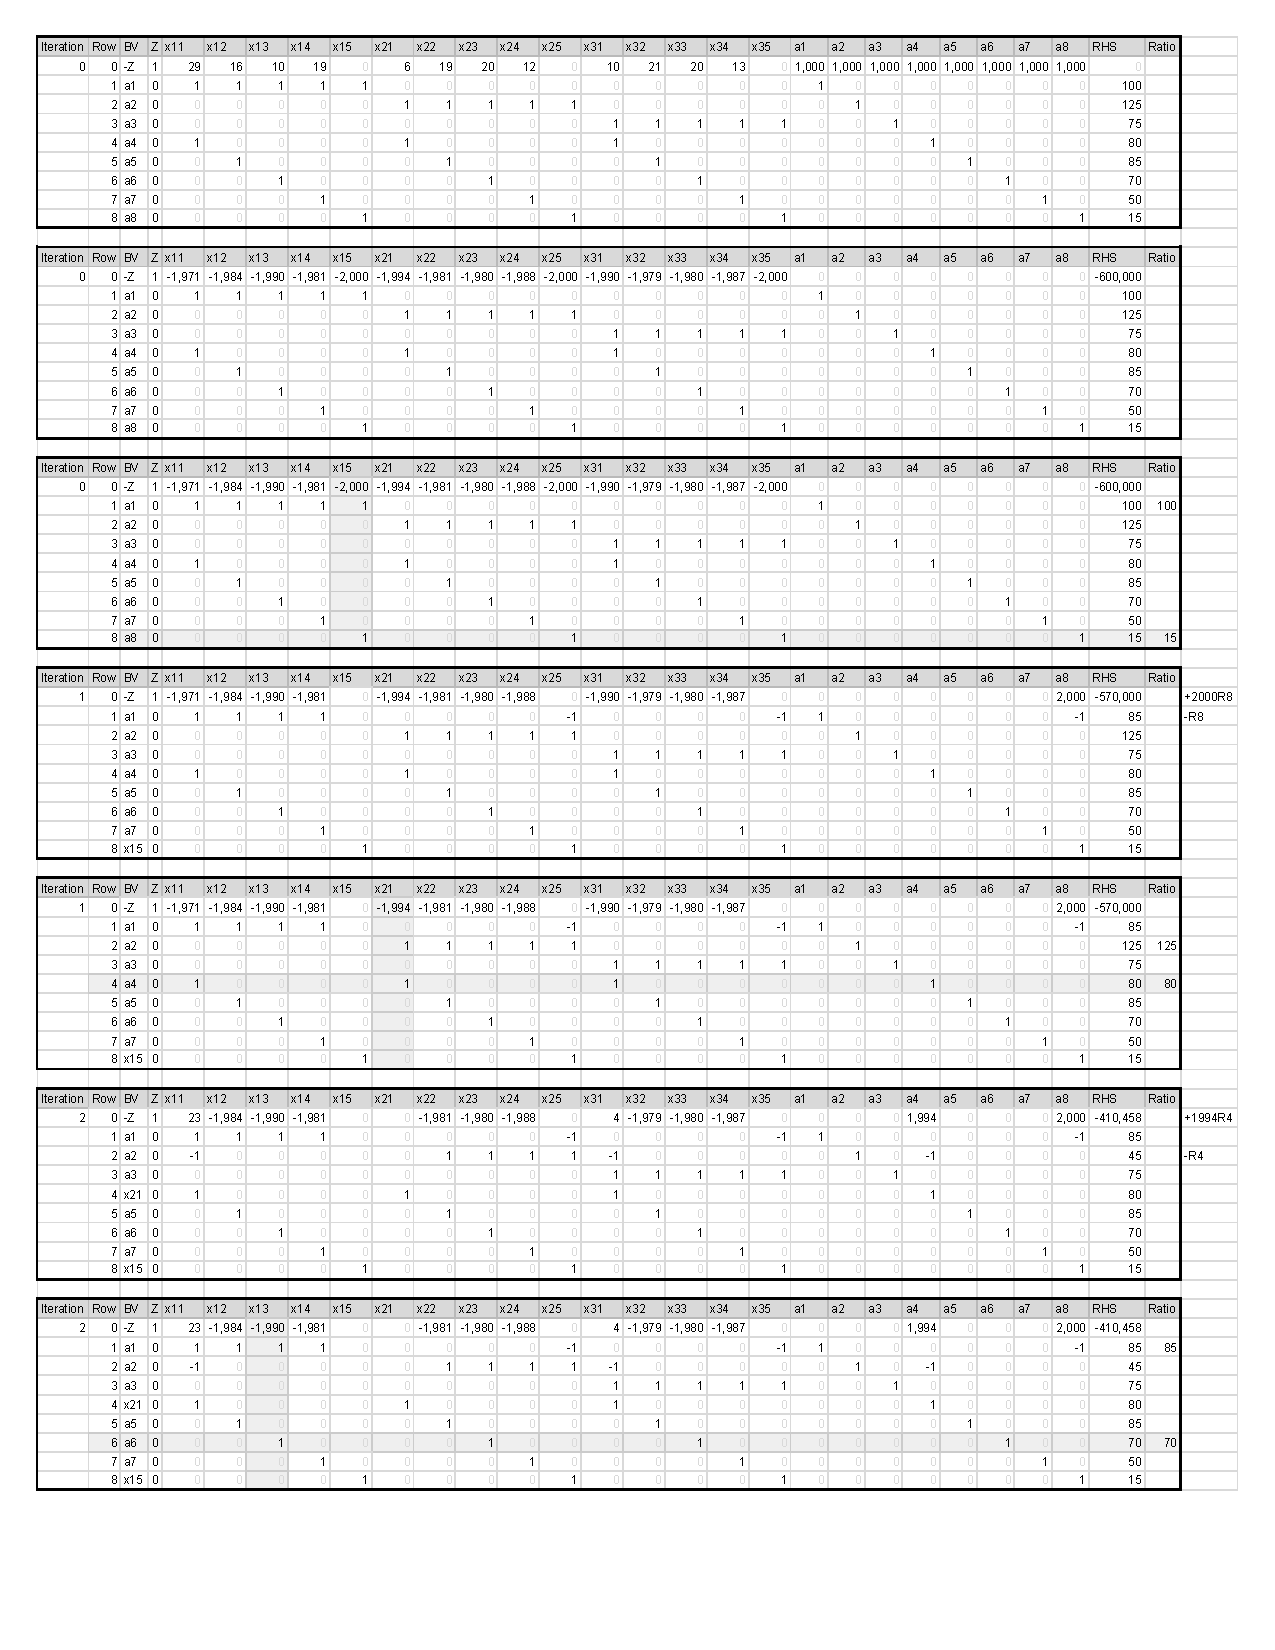
\includepdf[pages=-,pagecommand={},width=8.5in]{sheet.pdf}

With an approximate total distance of $Z = 3336$, we have obtained the following optimal solution:
\[
    x = \mqty[
        0 & 30 & 70 & 0 & 0 \\
        80 & 45 & 0 & 0 & 0 \\
        0 & 10 & 0 & 50 & 15
    ].
\]
Note that the fifth column is the dummy demand and does not appear on the map.

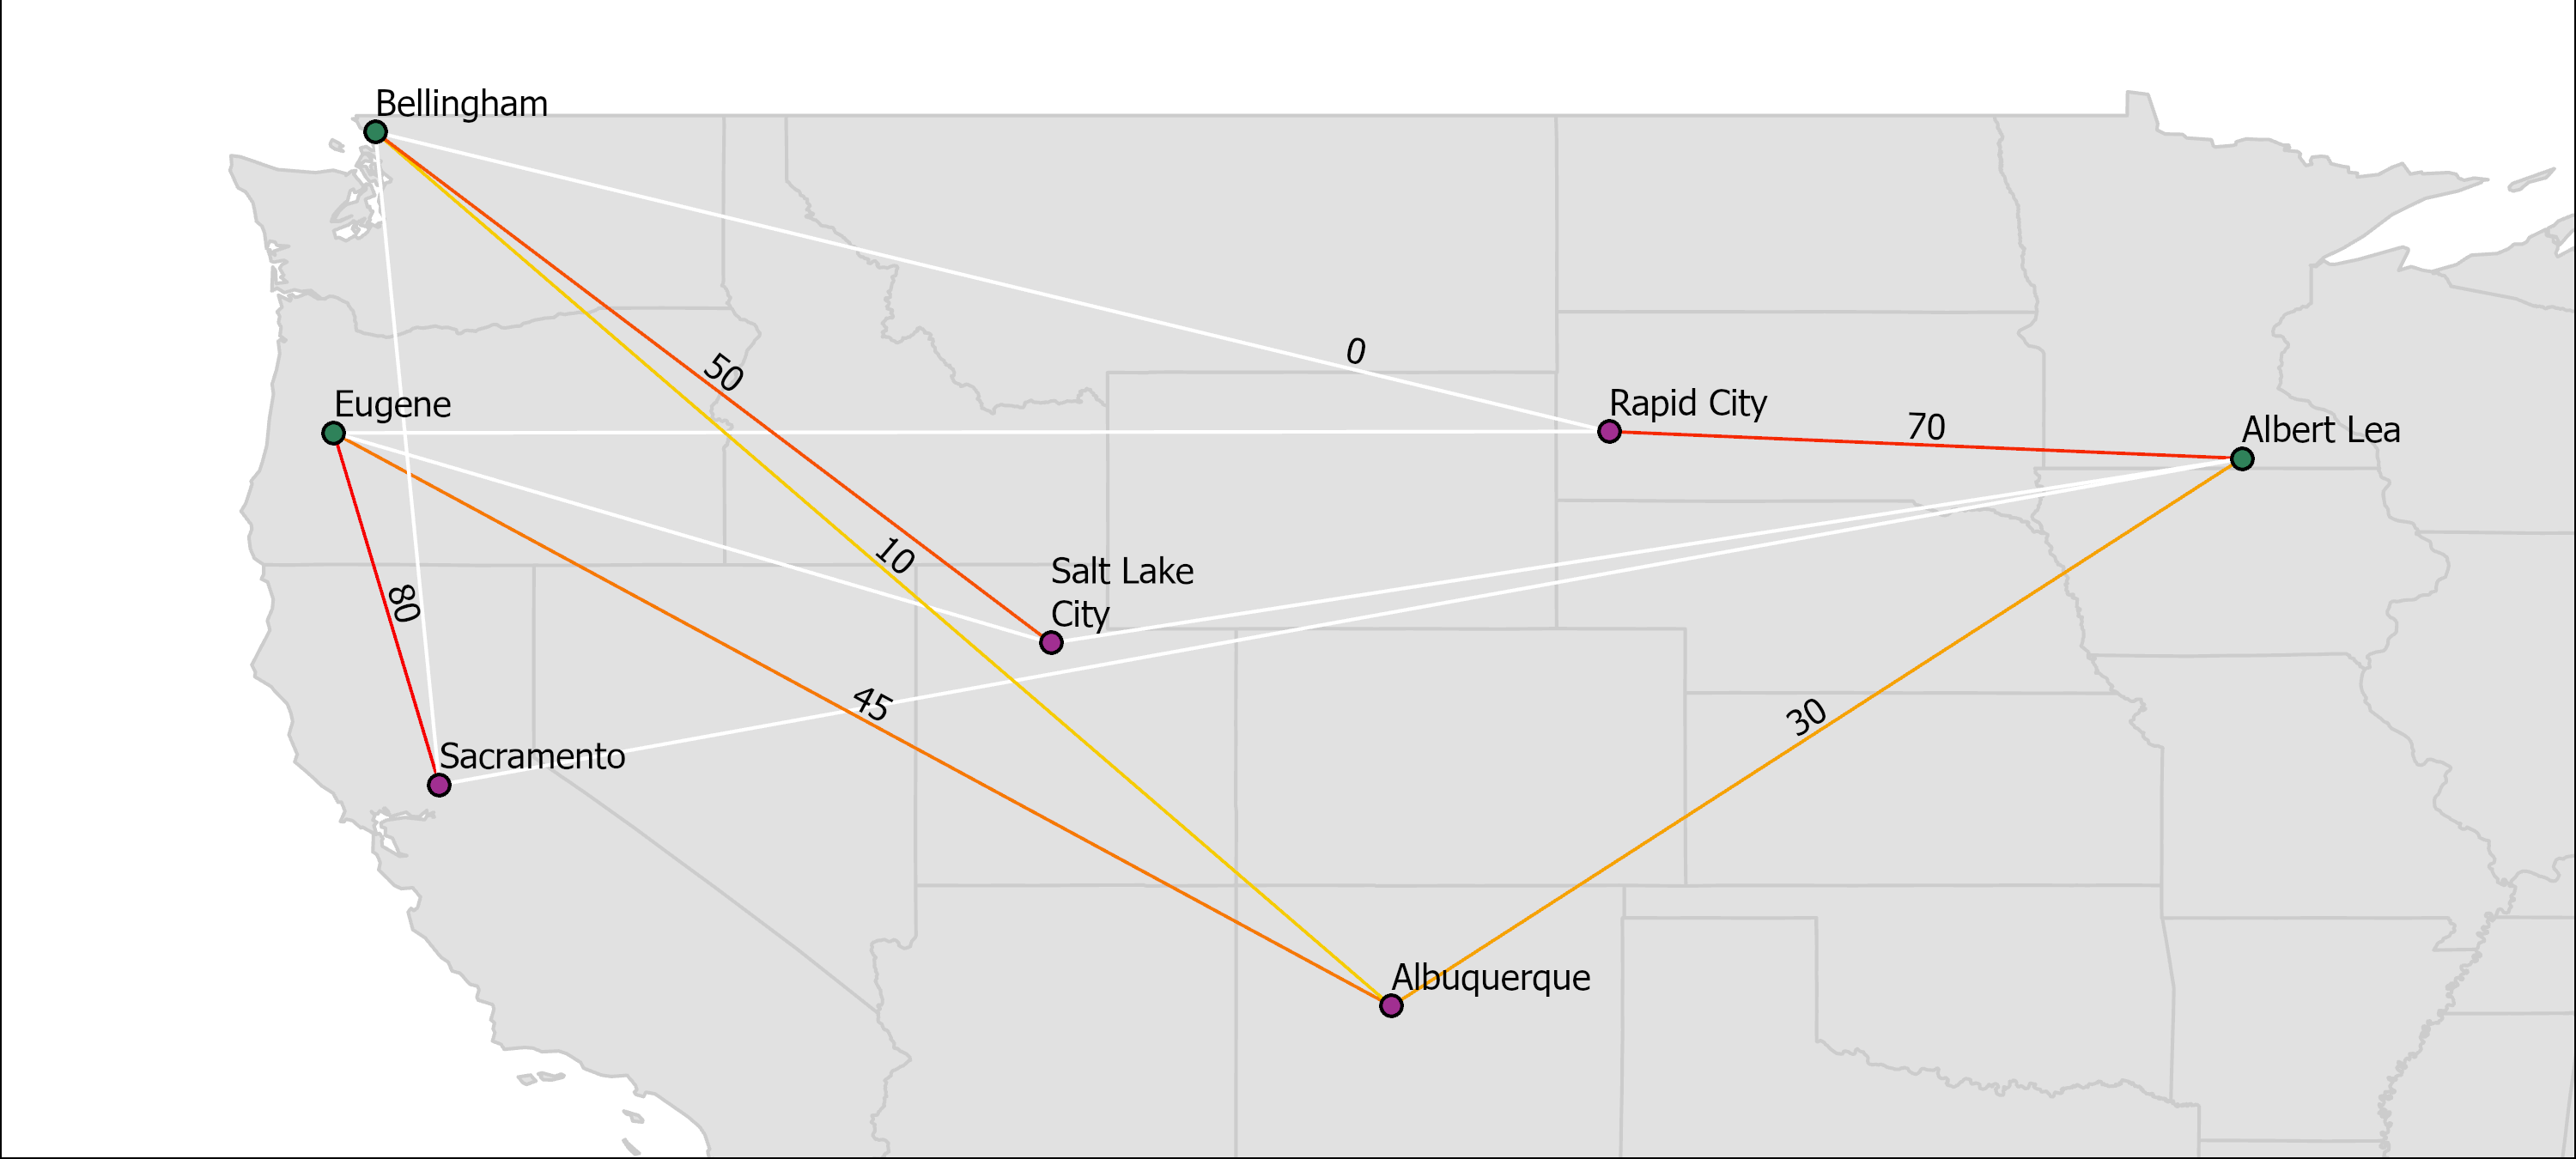
\includegraphics[width=\textwidth]{solmapmanual.png}

Total Dist: $3336$

\end{document}